\documentclass[12pt,letterpaper]{article}

% ---------- Paquetes ----------
\usepackage[spanish]{babel}
\usepackage[T1]{fontenc}
\usepackage[utf8]{inputenc}
\usepackage{geometry}
\geometry{margin=2.5cm}
\usepackage{booktabs}
\usepackage{tabularx}
\usepackage{array}
\usepackage{graphicx}
\graphicspath{{../graficas/}{../capturas/}}
\usepackage{subcaption}
\usepackage{amsmath,amssymb}
\usepackage{hyperref}
\hypersetup{colorlinks=true,linkcolor=blue,urlcolor=blue,citecolor=blue}
\usepackage{listings}
\usepackage{xcolor}
\usepackage{float}
\usepackage{caption}
\usepackage{parskip}
\usepackage{enumitem}
\usepackage{lmodern}
\usepackage{microtype}

\lstset{
  basicstyle=\small\ttfamily,
  backgroundcolor=\color{gray!10},
  frame=single,
  breaklines=true,
  numbers=left,
  numberstyle=\tiny\color{gray},
  keywordstyle=\color{blue}\bfseries,
  commentstyle=\color{green!60!black},
  stringstyle=\color{red!70!black},
  language=C
}

% ---------- Encabezado ----------
\title{\textbf{Lab 12 — ¿Por qué 8 núcleos no son $8\times$ más rápido?}\\
       \large Computación Paralela y Distribuida (CC3069)}
\author{Javier Eduardo España Pacheco\\
        \small Universidad del Valle de Guatemala\\[4pt]
        Repositorio: \url{https://github.com/Javier-Espana/LabSpeedUp-CPD.git}}
\date{Octubre 2026}

\begin{document}
\maketitle
\tableofcontents
\newpage

%------------------------------------------------------------------
\section{Datos del equipo}
%------------------------------------------------------------------

\subsection{Especificaciones de CPU}

\begin{table}[H]
\centering
\caption{Datos del procesador (obtenidos con \texttt{lscpu})}
\begin{tabularx}{\textwidth}{lX}
\toprule
\textbf{Campo} & \textbf{Valor} \\
\midrule
Modelo de CPU & AMD Ryzen 5 8400F 6-Core Processor \\
Arquitectura & x86\_64 \\
Familia / Modelo / Revisión & 25 / 117 / 2 \\
Núcleos físicos & 6 \\
Hilos por núcleo (SMT) & 2 \\
Núcleos lógicos (CPUs) & 12 \\
Núcleos de rendimiento/eficiencia & N/A (todos de rendimiento — AMD no usa big.LITTLE) \\
Hyper-Threading / SMT & Sí (2 hilos/núcleo) \\
Frecuencia máx. & 4{,}758 GHz \\
Turbo Boost & Habilitado \\
Caché L1d & 192 KiB (6 $\times$ 32 KiB) \\
Caché L1i & 192 KiB (6 $\times$ 32 KiB) \\
Caché L2 & 6 MiB (6 $\times$ 1 MiB, privada por núcleo) \\
Caché L3 & 16 MiB (compartida) \\
Virtualización & AMD-V \\
\bottomrule
\end{tabularx}
\end{table}

Con este hardware, \texttt{pmax = 12} (6 núcleos × 2 hilos SMT).

%------------------------------------------------------------------
\section{Parte 1 — La parte que no se puede repartir (Ley de Amdahl)}
%------------------------------------------------------------------

\subsection{Predicciones antes del experimento}

\textbf{Con \boldmath$f_p = 1.00$}: Todo el trabajo es paralelizable; la predicción de Amdahl es $S(12) = 12$. En la práctica espero un valor menor debido al overhead de crear y sincronizar hilos, y porque los núcleos SMT comparten recursos.

\textbf{Con \boldmath$f_p = 0.90$}: Aplicando la ley de Amdahl:
\[
S(12) = \frac{1}{1 - 0.90 + \dfrac{0.90}{12}} = \frac{1}{0.10 + 0.075} = \frac{1}{0.175} \approx 5.71
\]

\subsection{Resultados — Tabla Parte 1}

\begin{table}[H]
\centering
\caption{Speedup ($S$), eficiencia ($E$) y mejor $p$ para $F$ máxima. CPU: 12 hilos lógicos ($p_{\max}=12$).}
\begin{tabular}{rrrrrrr}
\toprule
$f_p$ & $S(p=2)$ & $S(p=4)$ & $S(p=12)$ & $E(p=12)$ & $p$ con $F$ máx \\
\midrule
1.00 & 1.983 & 3.958 & 8.233 & 0.686 & 11 \\
0.95 & 1.884 & 3.428 & 7.087 & 0.591 & 11 \\
0.90 & 1.799 & 3.056 & 5.487 & 0.457 & 10 \\
0.75 & 1.591 & 2.246 & 3.080 & 0.257 & 3  \\
0.50 & 1.311 & 1.570 & 1.786 & 0.149 & 1  \\
\bottomrule
\end{tabular}
\end{table}

\subsection{Cálculo a mano — dos filas}

\subsubsection*{Fila $f_p = 0.90$, $p = 4$}

De los datos CSV (\texttt{amdahl\_fp90.csv}):
\[
T_s = 0.496348\,\text{s}, \quad T_p(4) = 0.162429\,\text{s}
\]
\[
S = \frac{T_s}{T_p} = \frac{0.496348}{0.162429} = \mathbf{3.056}
\]
\[
E = \frac{S}{p} = \frac{3.056}{4} = \mathbf{0.764}
\]
\[
C = p \cdot T_p = 4 \times 0.162429 = \mathbf{0.6497}\,\text{hilo-s}
\]
\[
F = \frac{S}{C} = \frac{3.056}{0.6497} = \mathbf{4.703}\,\text{speedup/hilo-s}
\]

\subsubsection*{Fila $f_p = 1.00$, $p = 12$}

\[
T_s = 0.494336\,\text{s}, \quad T_p(12) = 0.060046\,\text{s}
\]
\[
S = \frac{0.494336}{0.060046} = \mathbf{8.233}
\]
\[
E = \frac{8.233}{12} = \mathbf{0.686}
\]
\[
C = 12 \times 0.060046 = \mathbf{0.7206}\,\text{hilo-s}
\]
\[
F = \frac{8.233}{0.7206} = \mathbf{11.425}\,\text{speedup/hilo-s}
\]

\subsection{Gráficas}

\begin{figure}[H]
\centering
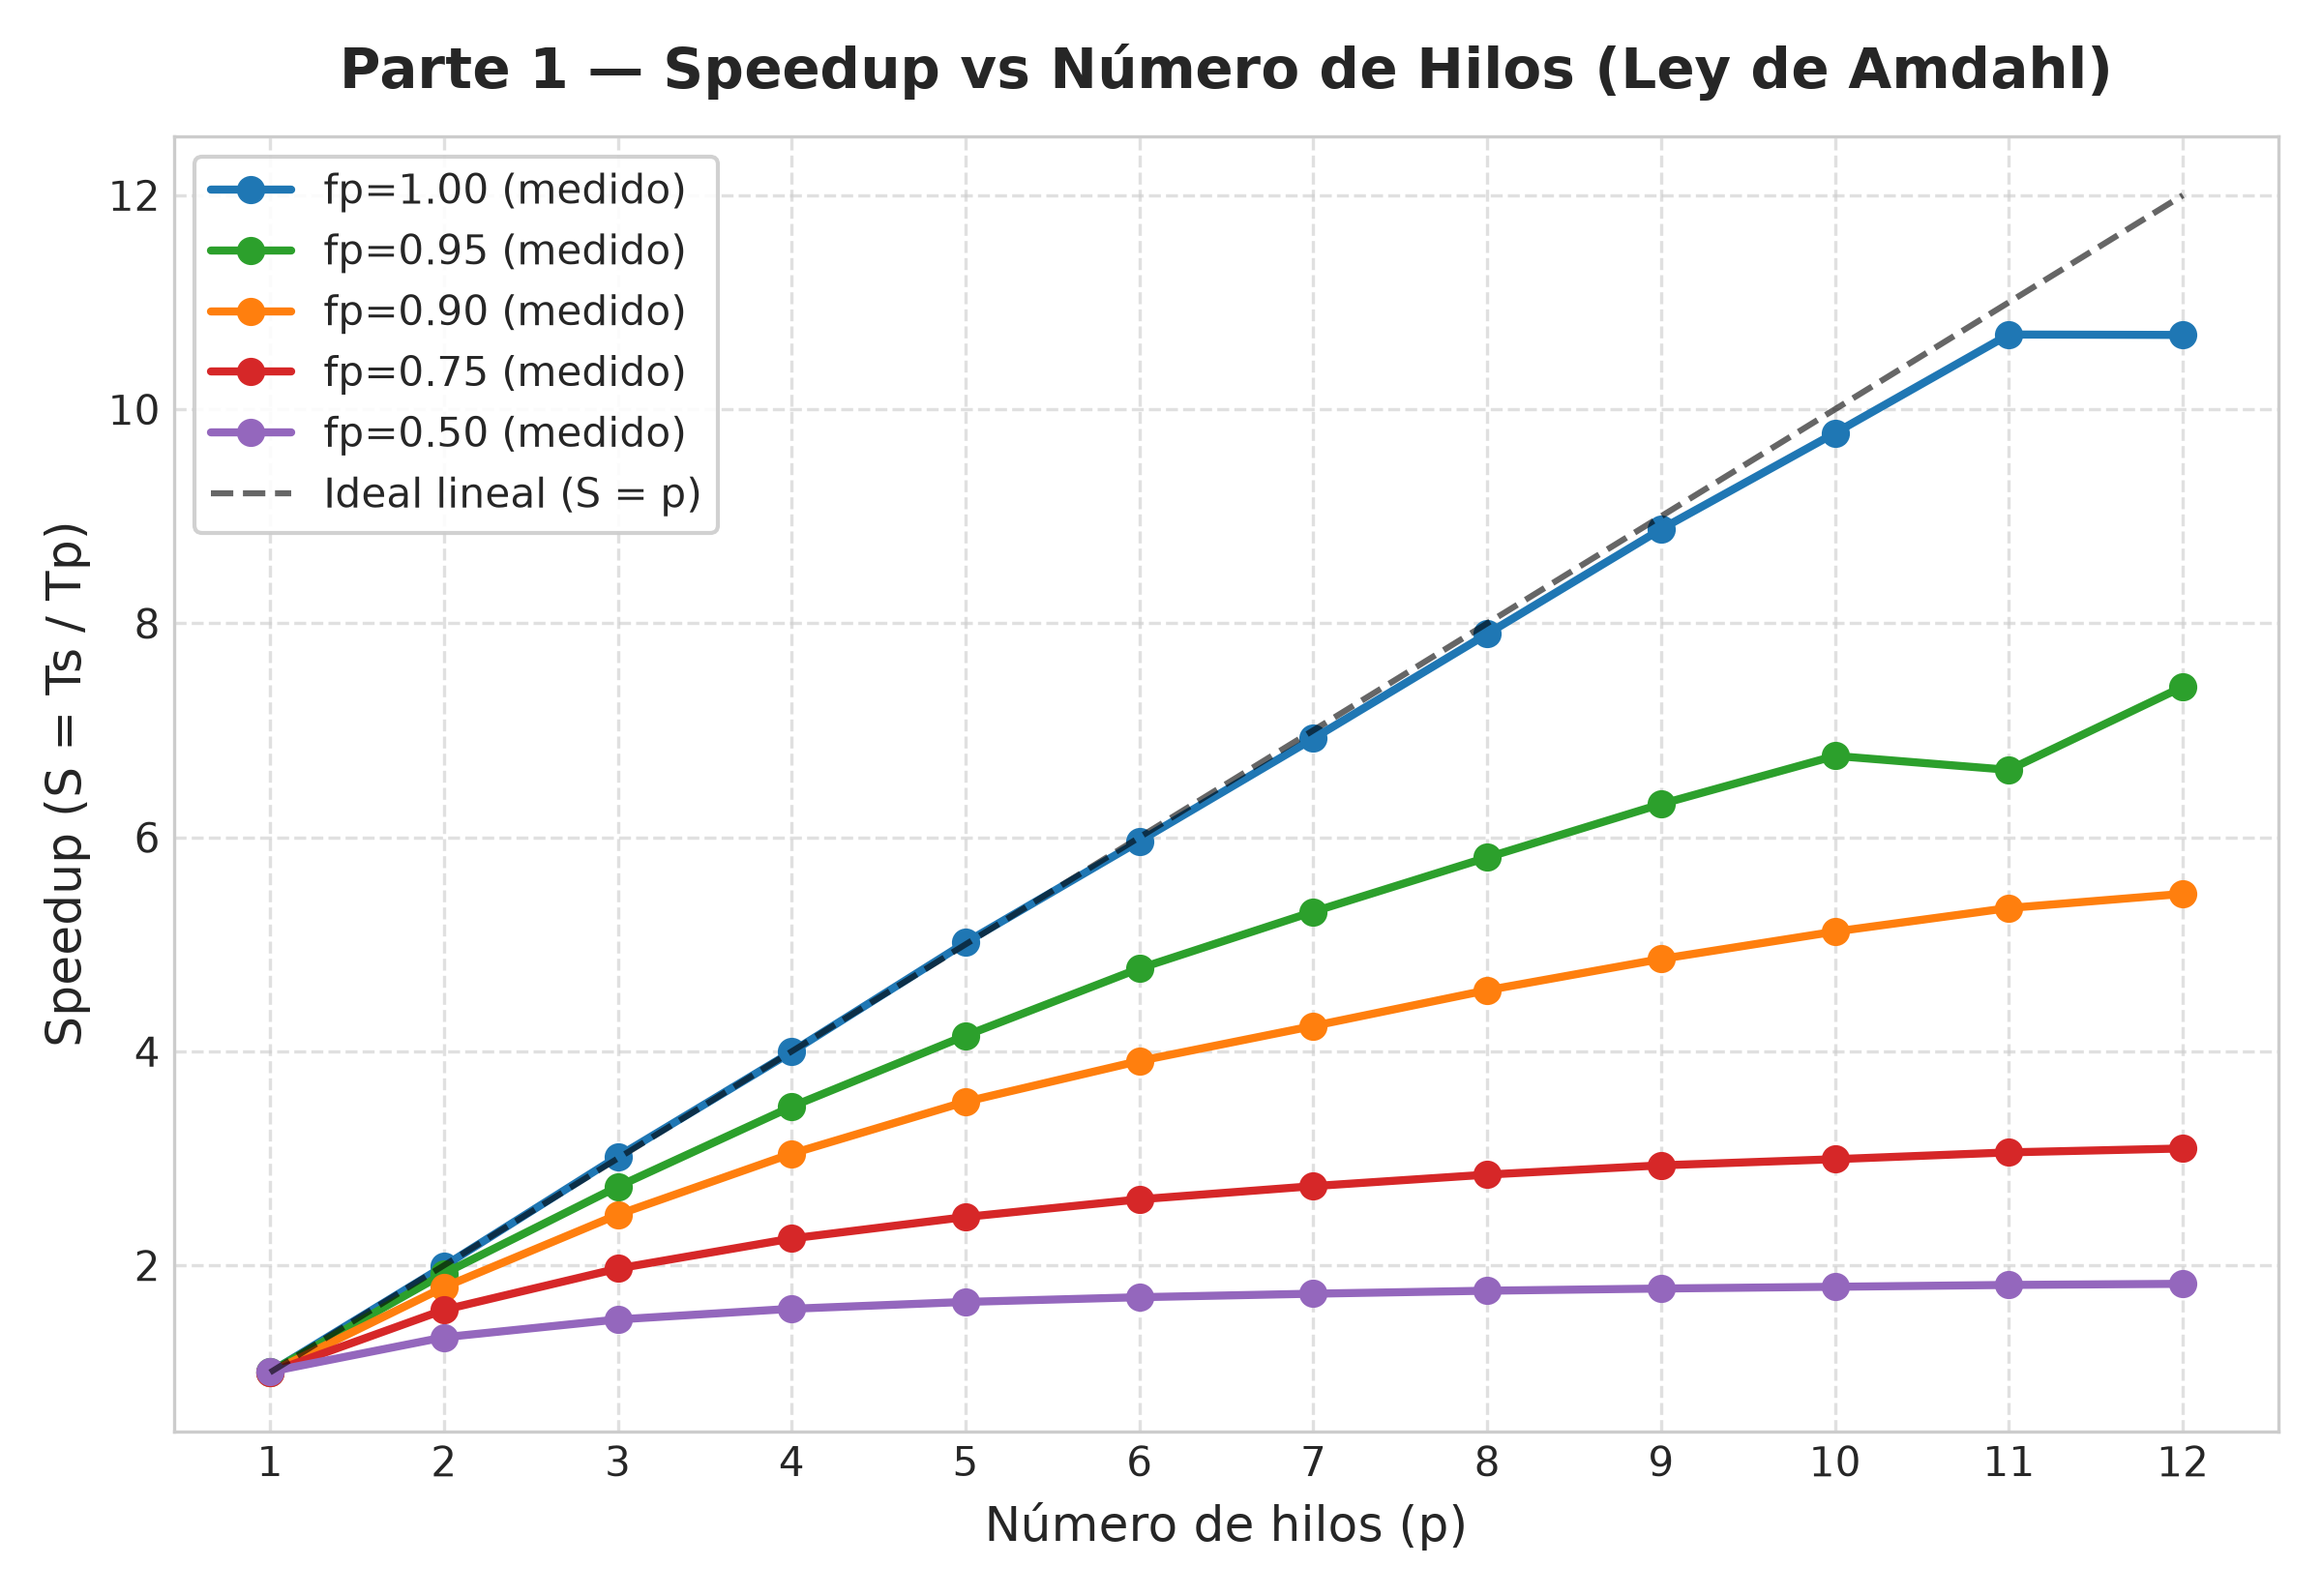
\includegraphics[width=0.80\textwidth]{grafica_amdahl_speedup.png}
\caption{Speedup vs. número de hilos para distintos valores de $f_p$.}
\end{figure}

\begin{figure}[H]
\centering
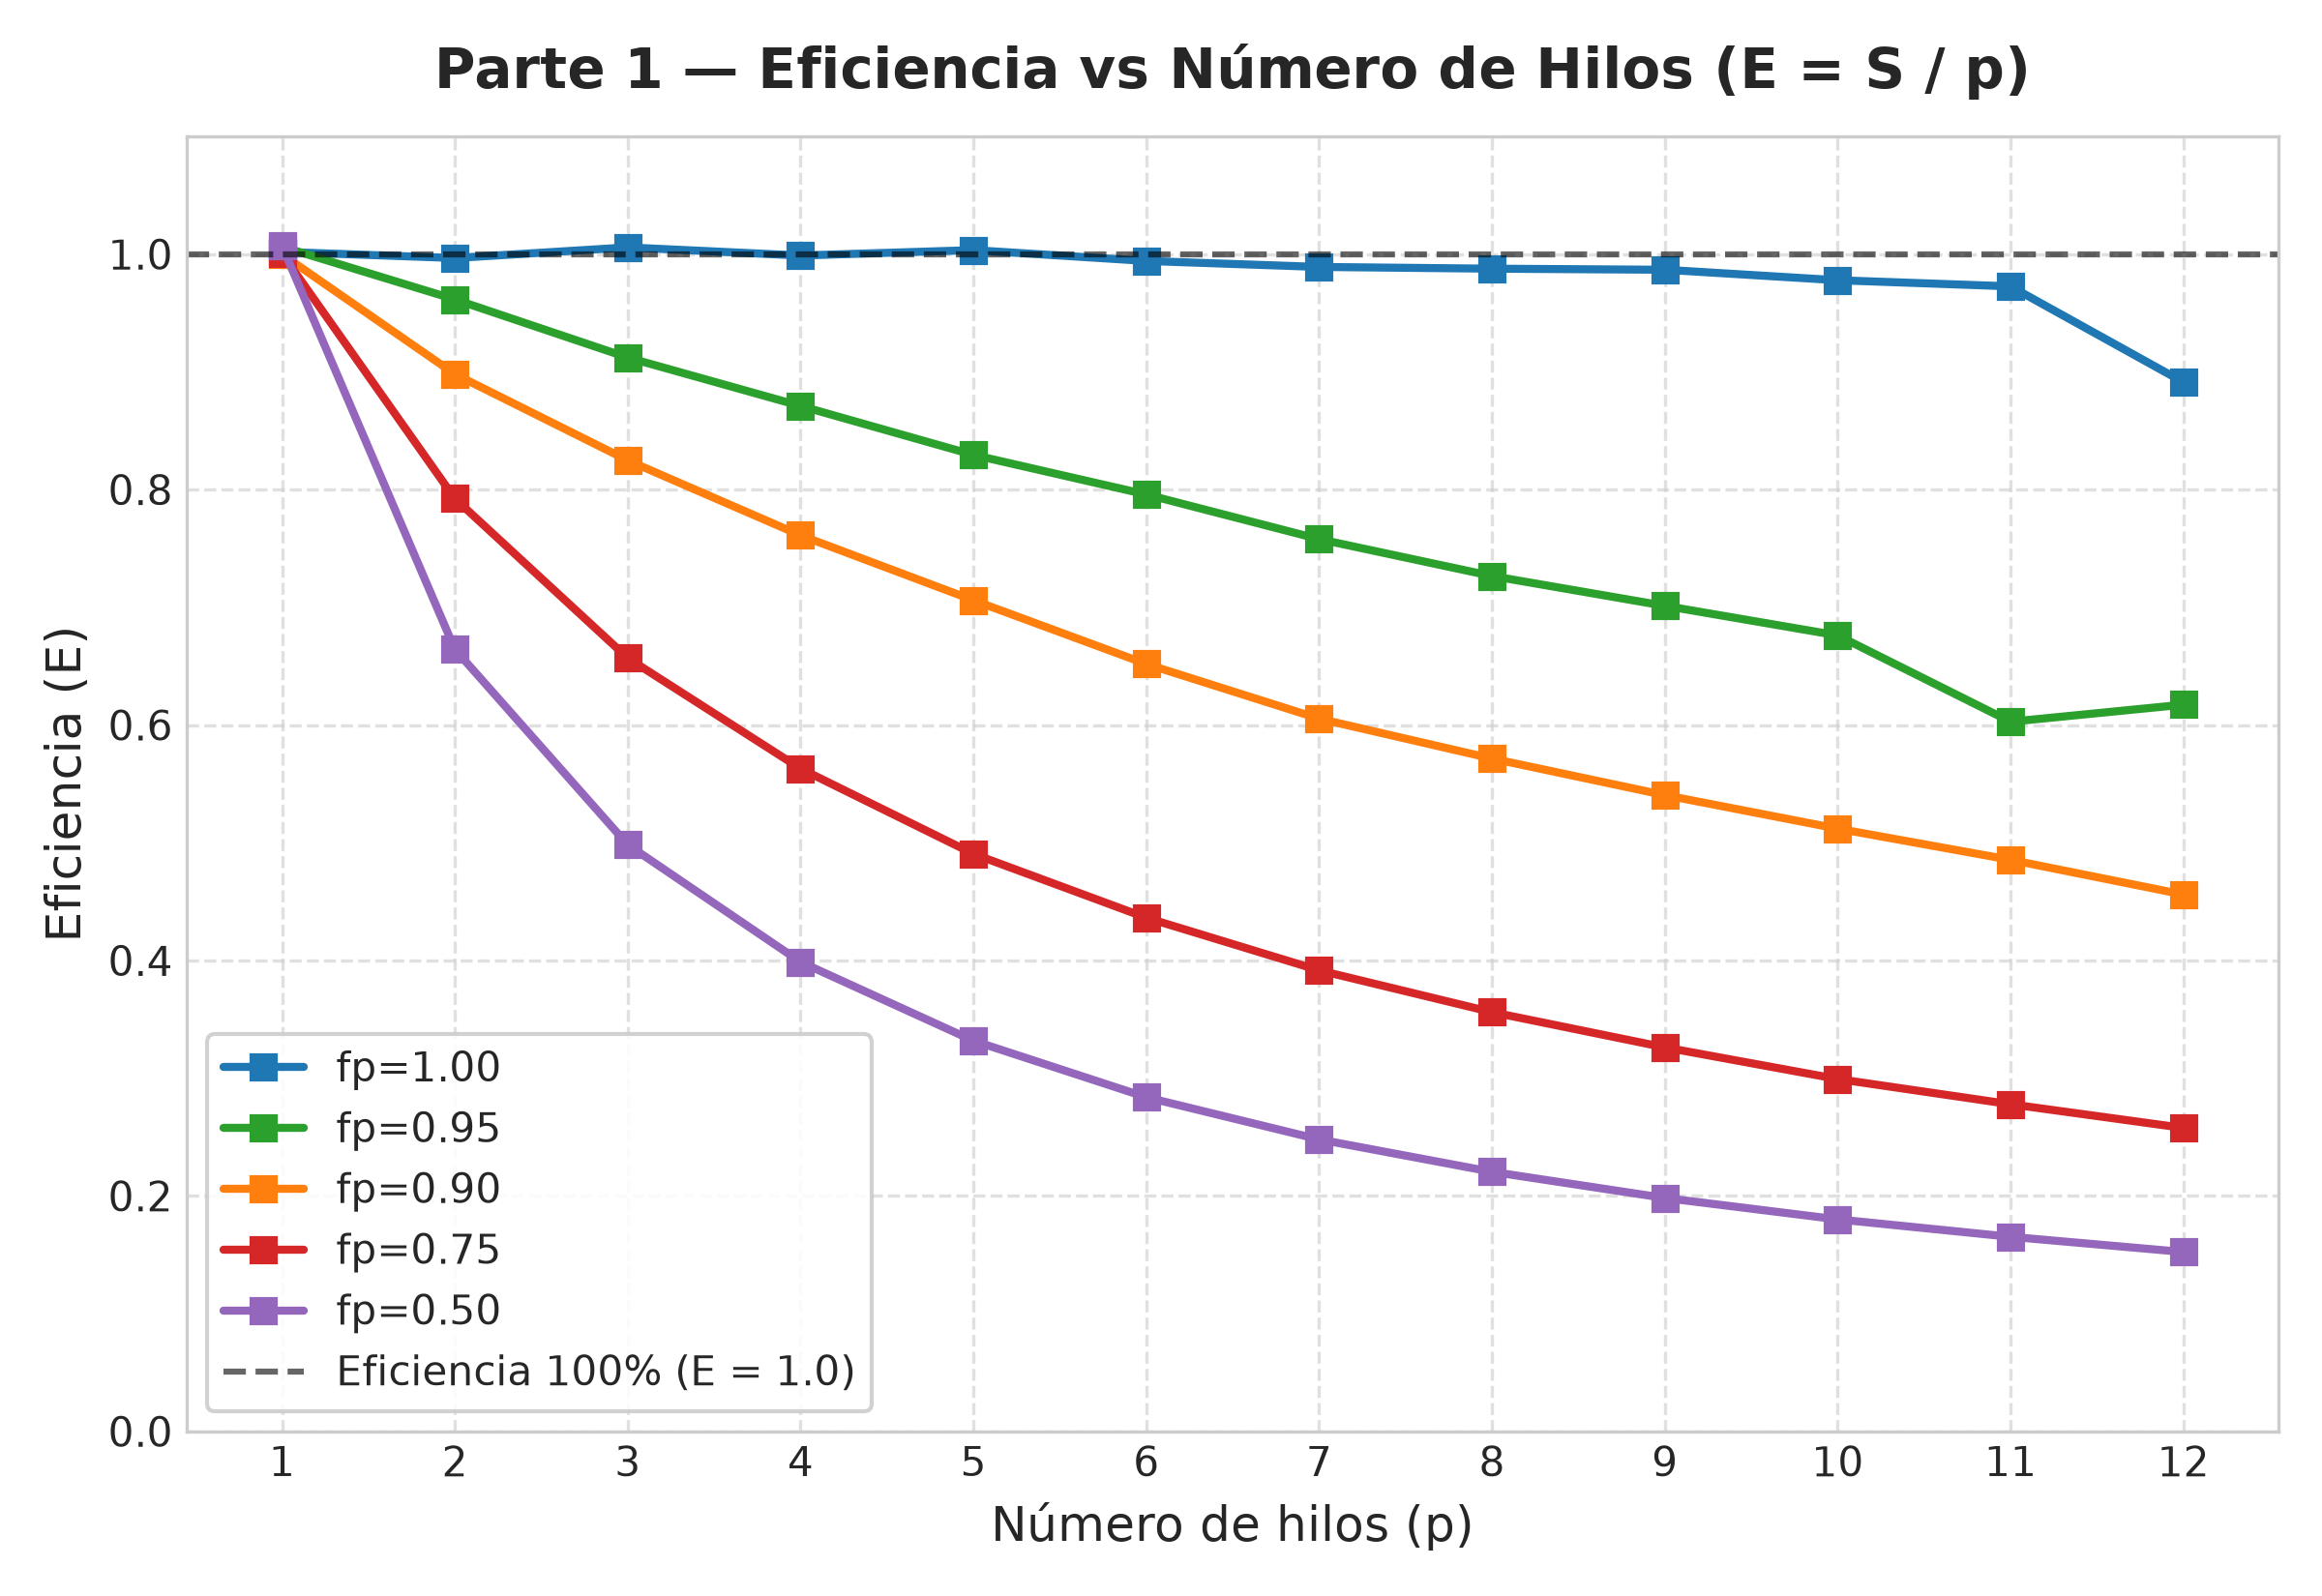
\includegraphics[width=0.80\textwidth]{grafica_amdahl_eficiencia.png}
\caption{Eficiencia $E = S/p$ vs. número de hilos.}
\end{figure}

\subsection{Preguntas}

\begin{enumerate}

\item \textbf{Con $f_p = 1.00$, ¿llegaste a $S = p$?}\\
No. Se midió $S(12) = 8.233$ en lugar del ideal $12$. Las causas son:
\begin{itemize}
  \item \textbf{Hyper-Threading (SMT):} los 6 núcleos físicos comparten recursos de ejecución entre sus 2 hilos lógicos (unidades de enteros, caché L1/L2). Al usar los 12 hilos lógicos, los 6 pares compiten por recursos → eficiencia degradada. Esto encaja en $\eta_c$ (overhead de sincronización y recursos compartidos).
  \item \textbf{Turbo Boost escalonado:} con un solo hilo la CPU puede alcanzar su máxima frecuencia ($\sim$4.76 GHz), pero con 12 hilos la potencia se reparte y la frecuencia baja a $\sim$4.1–4.3 GHz. Esto no encaja limpiamente en ninguna de las cuatro fugas estándar.
  \item \textbf{Overhead de creación/sincronización de hilos:} barrera implícita al final del \texttt{parallel for}. Encaja en $\eta_c$.
\end{itemize}

\item \textbf{Forma de la curva con $f_p = 0.75$:}\\
La curva sube rápido al principio pero pronto se aplana. La ganancia de pasar de 1 a 2 hilos es $\approx 0.59$, pero de 11 a 12 hilos es prácticamente cero ($S$ casi no cambia). La fracción secuencial del 25\% domina y limita el speedup máximo teórico a $1/0.25 = 4.0$, que nunca se alcanza.

\item \textbf{Derivación del modelo (Ley de Amdahl):}\\
Un programa tarda $T_1$ en un núcleo. La fracción $f_p$ se divide en $p$ hilos y la fracción $(1-f_p)$ es secuencial:
\[
T_p = (1 - f_p)\,T_1 + \frac{f_p \cdot T_1}{p}
\]
\[
S(p) = \frac{T_1}{T_p} = \frac{T_1}{(1-f_p)T_1 + \dfrac{f_p T_1}{p}} = \frac{1}{(1-f_p) + \dfrac{f_p}{p}}
\]

\item \textbf{Predicción con el modelo vs. lo medido ($f_p = 0.90$, $p = 12$):}\\
\[
S_{\text{modelo}}(12) = \frac{1}{0.10 + 0.90/12} = \frac{1}{0.10 + 0.075} = \frac{1}{0.175} \approx 5.71
\]
Medido: $S = 5.487$. Diferencia de $\approx 4\%$; el modelo sobreestima ligeramente porque no considera el overhead de SMT ni la reducción de frecuencia.

\item \textbf{Límite cuando $p \to \infty$ con $f_p = 0.90$:}\\
\[
\lim_{p\to\infty} S(p) = \frac{1}{1 - f_p} = \frac{1}{0.10} = \mathbf{10}
\]
Con 1000 núcleos el speedup máximo posible sería $\approx 10$, no 1000.

\item \textbf{Despejando $f_p$ real del speedup medido:}\\
$S_{\text{medido}} = 5.487$, $p = 12$:
\[
5.487 = \frac{1}{(1-f_p) + f_p/12} \Rightarrow (1-f_p) + f_p/12 = \frac{1}{5.487} = 0.1822
\]
\[
1 - f_p + f_p/12 = 0.1822 \Rightarrow 1 - 0.9167\,f_p = 0.1822 \Rightarrow f_p = \frac{0.8178}{0.9167} \approx 0.892
\]
El $f_p$ efectivo medido es $\approx 0.892 < 0.90$. La diferencia ($0.008$) representa las fugas $\eta_c$ (overhead de sincronización).

\item \textbf{Efectividad $F$ con $f_p = 0.90$:}\\
$F$ es máxima con $p = 10$ ($F = 5.33$). Este no es el mismo $p$ que da el menor tiempo ($p = 12$, $T_p = 0.090\,\text{s}$). Con $p = 10$ se obtiene el mejor balance entre rapidez y costo. Con 16 números en clase el óptimo era $p = 4$; aquí el problema más grande desplaza el óptimo a $p$ mayor.

\item \textbf{Servidor de 64 núcleos para un programa de 20 s con 2 s secuenciales:}\\
$f_p = 18/20 = 0.90$, fracción secuencial $= 0.10$.
\[
S(64) = \frac{1}{0.10 + 0.90/64} = \frac{1}{0.10 + 0.01406} \approx 8.82
\]
\[
E(64) = \frac{8.82}{64} \approx 0.138
\]
\textbf{Respuesta:} el servidor de 64 núcleos solo daría $\approx8.8\times$ de speedup (no $64\times$), con una eficiencia muy baja del 13.8\%. Solo se justifica si el costo del servidor es bajo; de lo contrario, un servidor de 8–10 núcleos con $E \approx 0.50$ sería más costo-efectivo.

\end{enumerate}

%------------------------------------------------------------------
\section{Parte 2 — ¿Vale la pena paralelizar algo pequeño?}
%------------------------------------------------------------------

\subsection{2a. El $T_s$ honesto}

De \texttt{amdahl\_fp100.csv}, fila $p = 1$:
\begin{itemize}
  \item \texttt{t\_seq} = 0.494336 s (versión sin OpenMP)
  \item \texttt{t\_par} con $p=1$ = 0.493555 s (OpenMP, 1 hilo)
\end{itemize}

\textbf{1.} En esta máquina \texttt{t\_par}($p=1$) es prácticamente igual a \texttt{t\_seq} ($\Delta \approx 0.16\%$). El overhead de inicializar el entorno OpenMP es insignificante para trabajos grandes.

\textbf{2.} Si se usa como $T_s$ el tiempo del programa paralelo con 1 hilo, el speedup sale \emph{inflado}: se divide un tiempo ya penalizado por el overhead OpenMP entre el tiempo con $p$ hilos. El speedup "real" de mejora hardware es menor, pero el numerador está artificialmente hinchado. Es tramposo porque oculta que el paralelismo mismo introduce un costo.

\subsection{2b. Sumar N números}

\textbf{Predicción:} Para $N$ pequeño (16, 1024) la versión paralela será más lenta. El overhead de OpenMP (despertar hilos, barrera, reduction) tarda cientos de nanosegundos, mientras que sumar 16 doubles tarda $\sim$3 ns. Estimo que la versión paralela comienza a ganar a partir de $N \approx 65{,}536$ (64K elementos).

\begin{figure}[H]
\centering
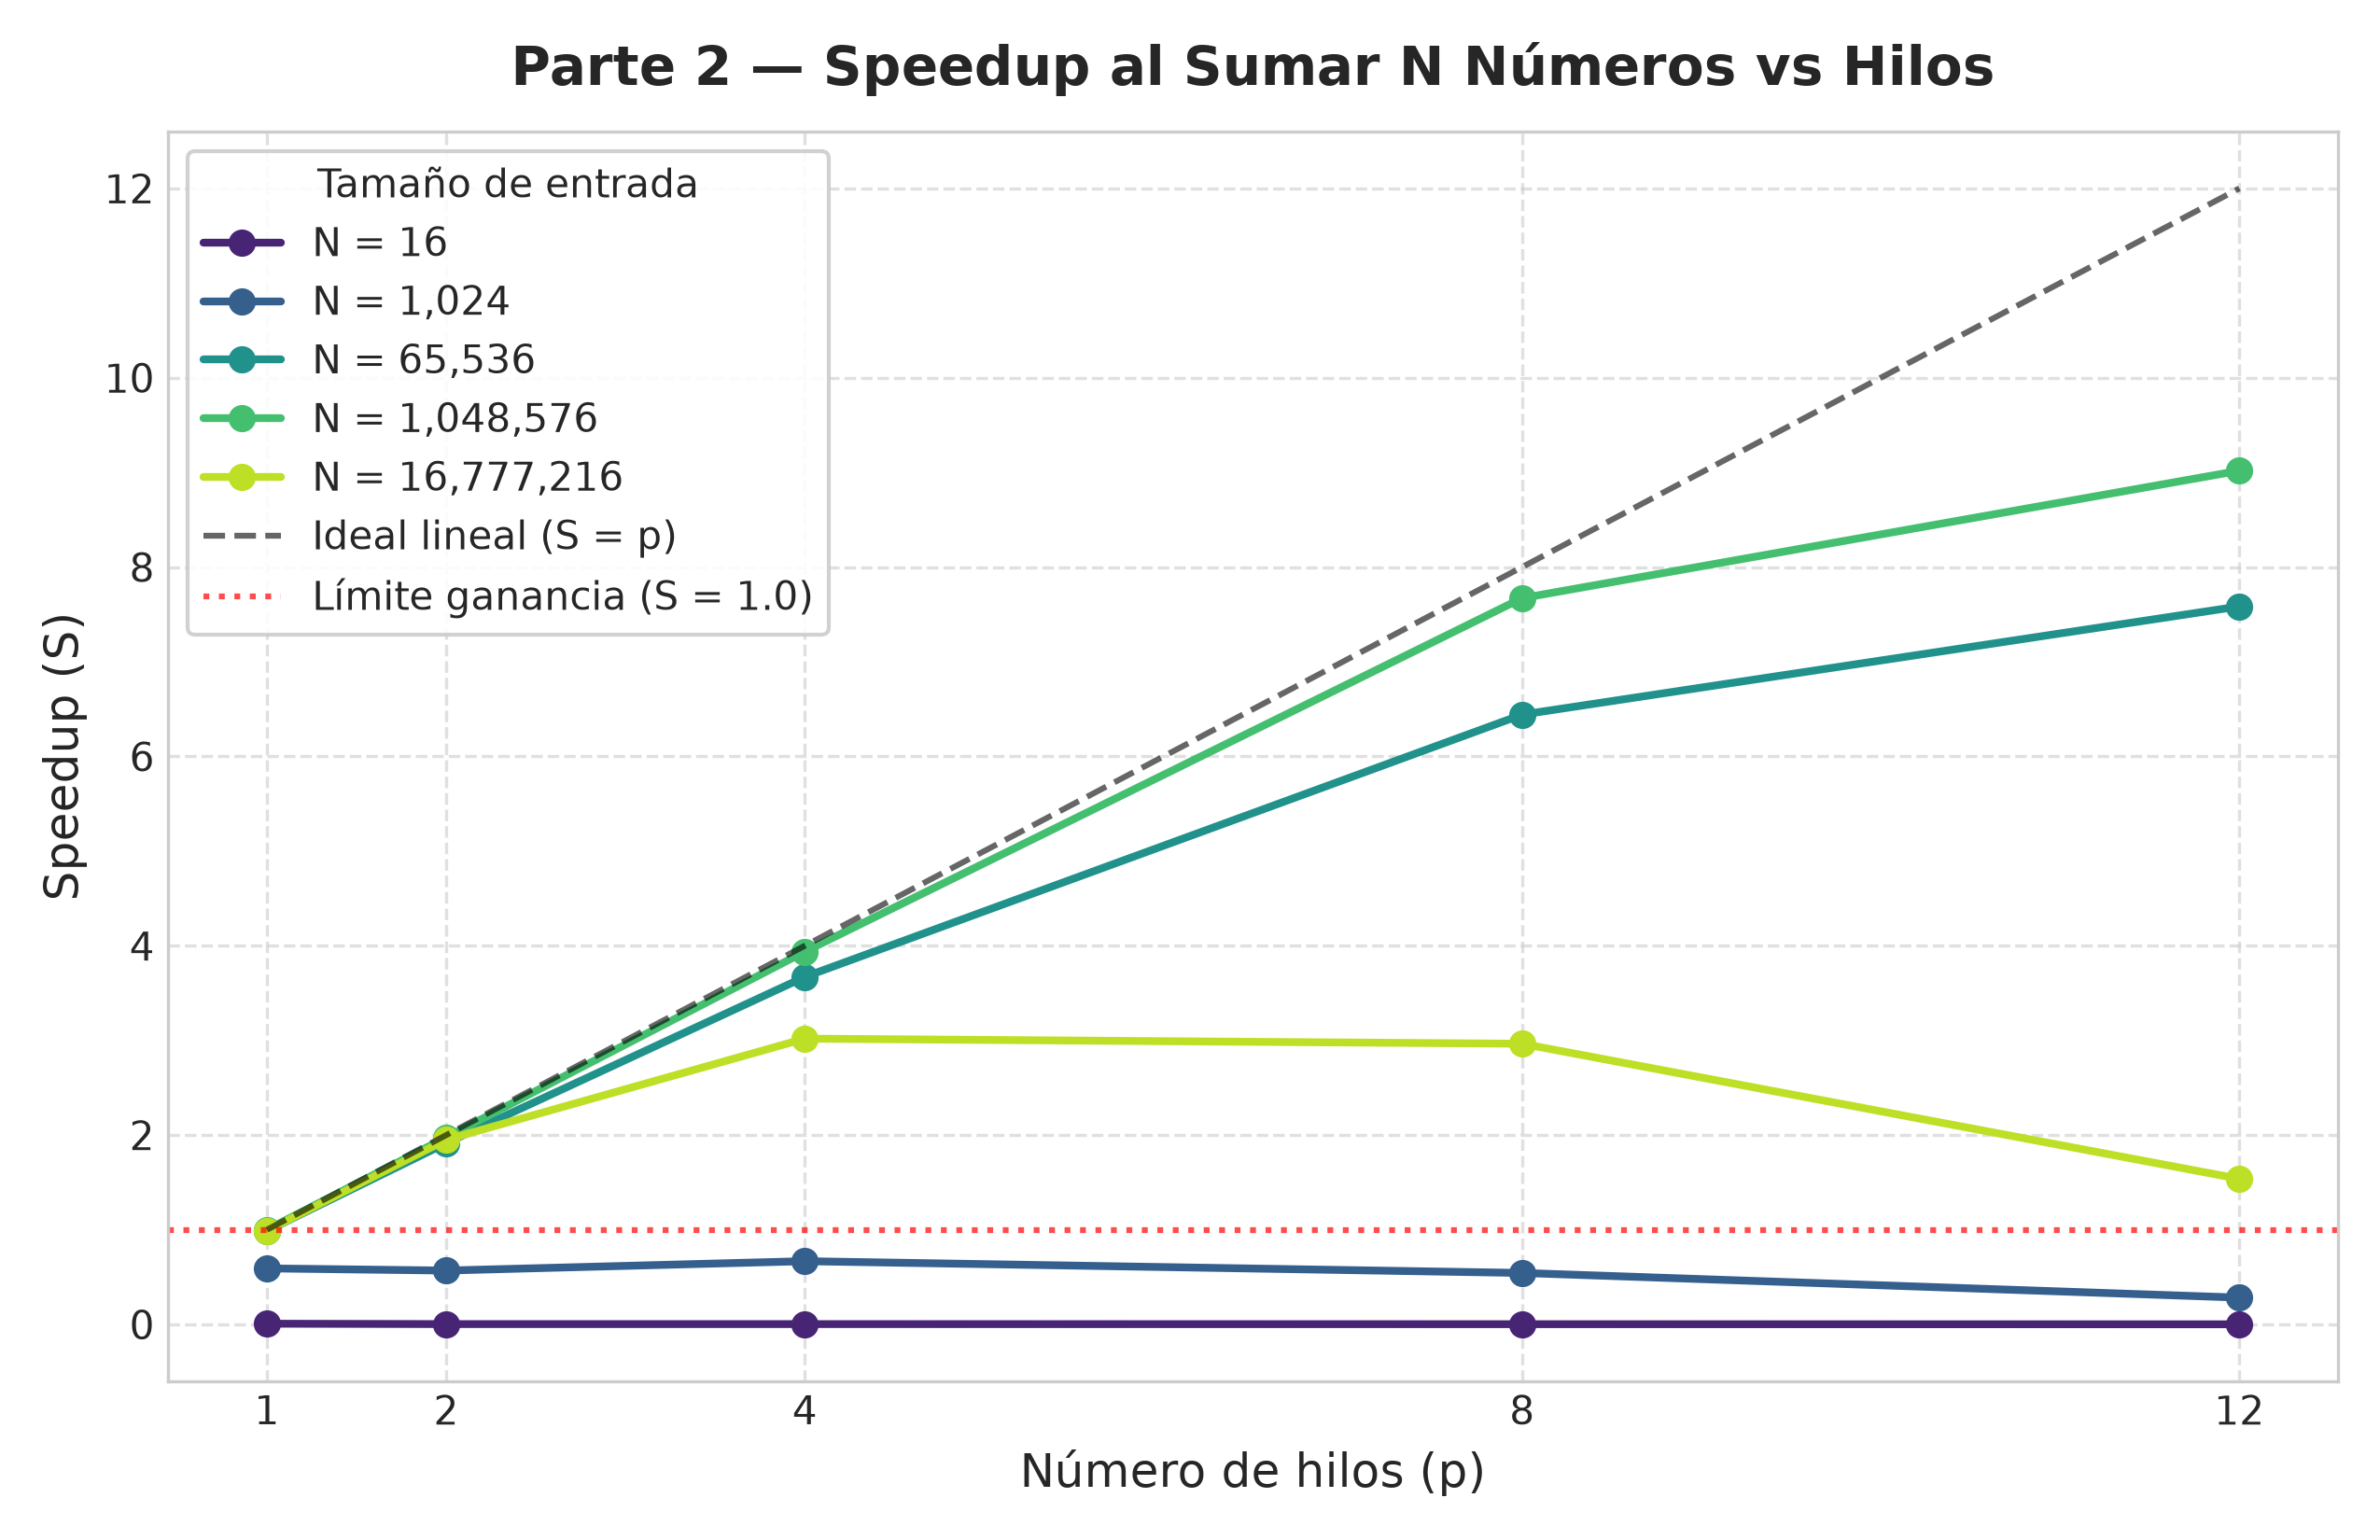
\includegraphics[width=0.80\textwidth]{grafica_suma_speedup.png}
\caption{Speedup al sumar $N$ números con distintos tamaños de entrada.}
\end{figure}

\begin{figure}[H]
\centering
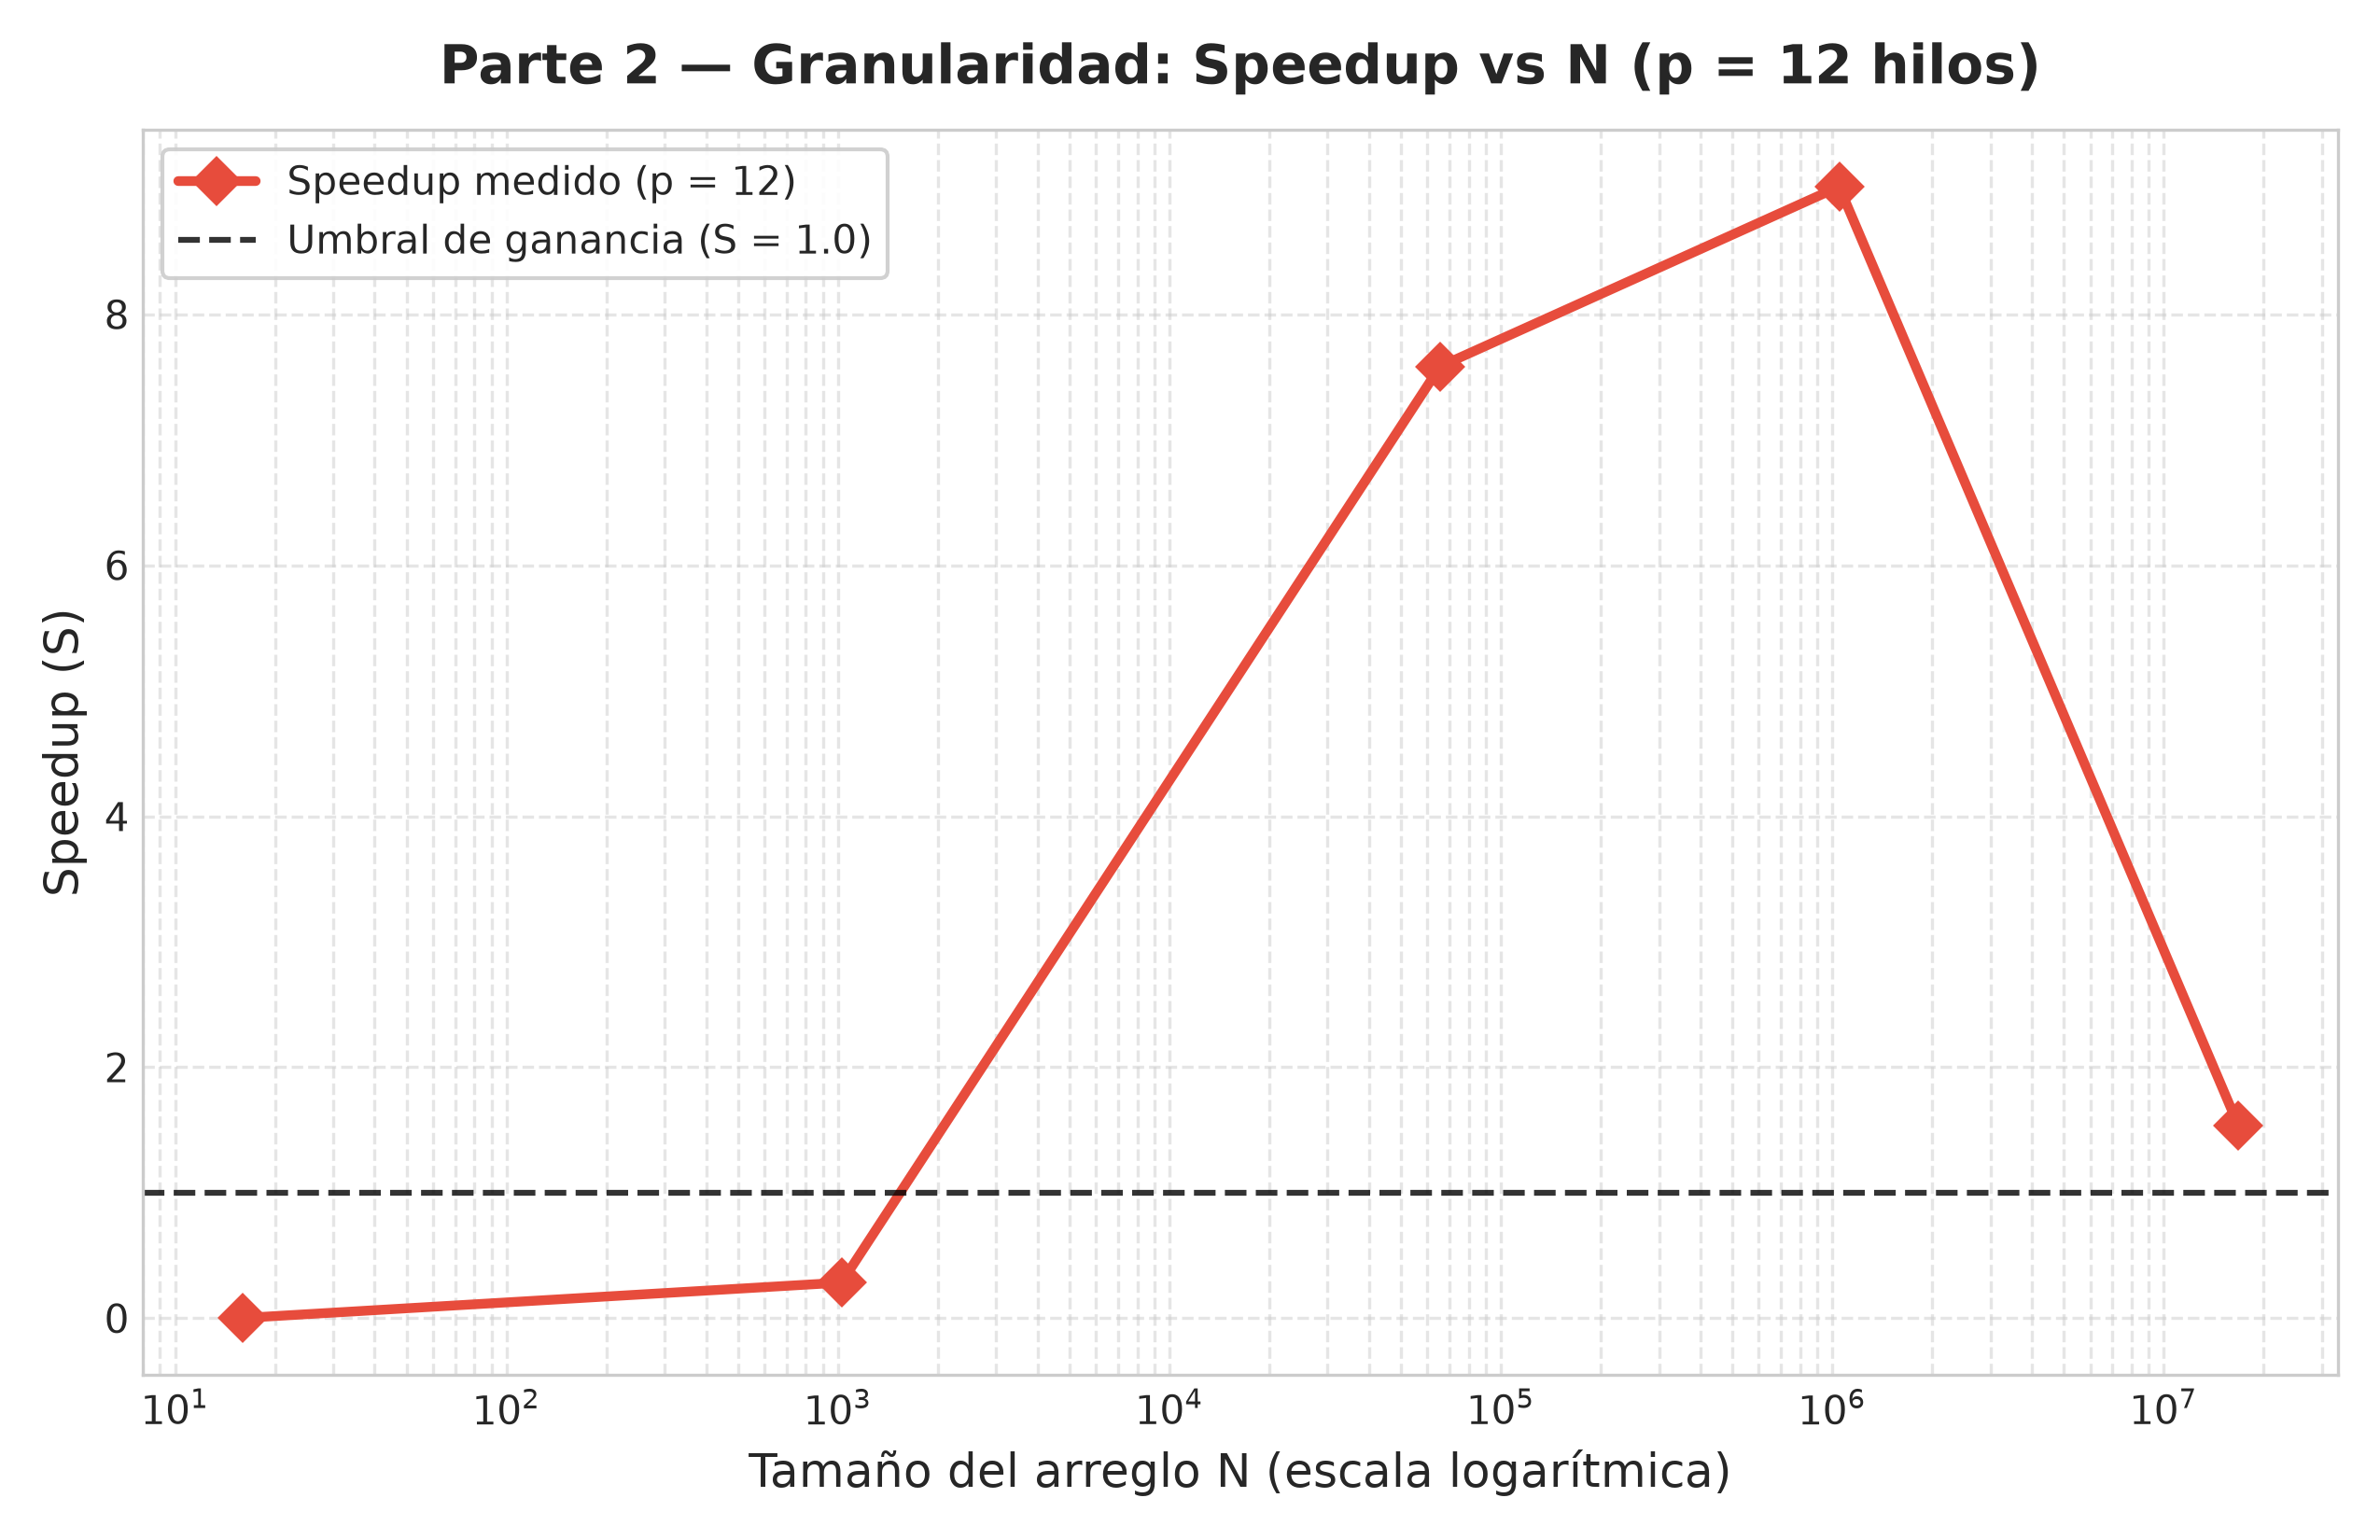
\includegraphics[width=0.80\textwidth]{grafica_suma_granularidad.png}
\caption{Granularidad: speedup vs.\ $N$ con $p = 12$ hilos.}
\end{figure}

\begin{enumerate}[start=3]

\item \textbf{$N=16$, $p=12$: ¿cuánto vale $S$?}\\
$T_s = 3\,\text{ns}$, $T_p = 1755\,\text{ns}$: $S = 3/1755000 \approx \mathbf{0.0017}$.\\
La versión paralela es $\approx \mathbf{585}$ veces \emph{más lenta}.

\item \textbf{Supuesto del modelo de dos fases que no se cumple:}\\
El modelo asume que el costo de sincronización (despertar hilos, barrera, reduction en árbol) es igual a "1 suma". En la práctica, despertar los 12 hilos cuesta cientos de microsegundos, mientras que cada suma individual tarda $\sim$0.2 ns. El supuesto violado es que \textbf{el overhead de comunicación/sincronización es despreciable}. La fuga es $\eta_c$ (comunicación y sincronización).

\item \textbf{Lo que OpenMP hace en cada \texttt{parallel for} (aparte de sumar):}\\
Despertar hilos desde el pool, asignar iteraciones a cada hilo, ejecutar la suma local, combinar los resultados parciales (\texttt{reduction}), esperar en la barrera implícita, y devolver el control al hilo maestro. Con $N=16$ en $\sim$3 ns, todo ese overhead ($\sim$1{,}000–2{,}000 ns) domina.

\item \textbf{¿A partir de qué $N$ conviene paralelizar?}\\
Del CSV: la versión paralela supera a la secuencial en $N = 65{,}536$ ($S \approx 3.68$ con $p=4$, $S \approx 7.23$ con $p=12$). \textbf{Regla práctica:} un \texttt{parallel for} solo conviene cuando cada iteración cuesta al menos $\sim$1–10 µs, o cuando $N$ es suficientemente grande para que el trabajo por hilo supere en varios órdenes de magnitud el overhead de sincronización ($\sim$1–2 µs).

\item \textbf{$N$ grande: ¿llega $S$ a $p$?}\\
No del todo. Con $N = 1{,}048{,}576$ y $p = 8$: $S \approx 7.76$. Con $N = 16{,}777{,}216$ el speedup baja a $S \approx 2.88$ con $p = 4$ y $S \approx 2.84$ con $p = 8$. La suma tiene una razón aritmética/memoria muy baja: solo una suma por cada dato cargado. El \textbf{ancho de banda de memoria} (compartido entre núcleos vía el bus) limita el speedup. Esto no encaja exactamente en ninguna de las cuatro fugas clásicas ($\eta_f, \eta_c, \eta_b, \eta_r$); es una limitación de \emph{ancho de banda de memoria} (memory bandwidth bound).

\end{enumerate}

%------------------------------------------------------------------
\section{Parte 3 — Cuando a un hilo le toca más trabajo (Desbalance)}
%------------------------------------------------------------------

\subsection{Predicción}

Con $p = 4$ y \texttt{static}: el rango $[0, W-1]$ se divide en 4 bloques contiguos iguales. El costo de la iteración $i$ crece como una función lineal. El hilo 3 (bloque $[3W/4, W-1]$) tiene el trabajo más costoso: el área de su trapecio es $\approx 87.5\%$ del trabajo total dividido por 4, mientras que el hilo 0 solo tiene $\approx 12.5\%/1 = 12.5\%$. El hilo más cargado tarda $\approx 3.5\times$ más que el menos cargado → speedup esperado $\approx 4/3.5 \approx 1.14$.

\begin{figure}[H]
\centering
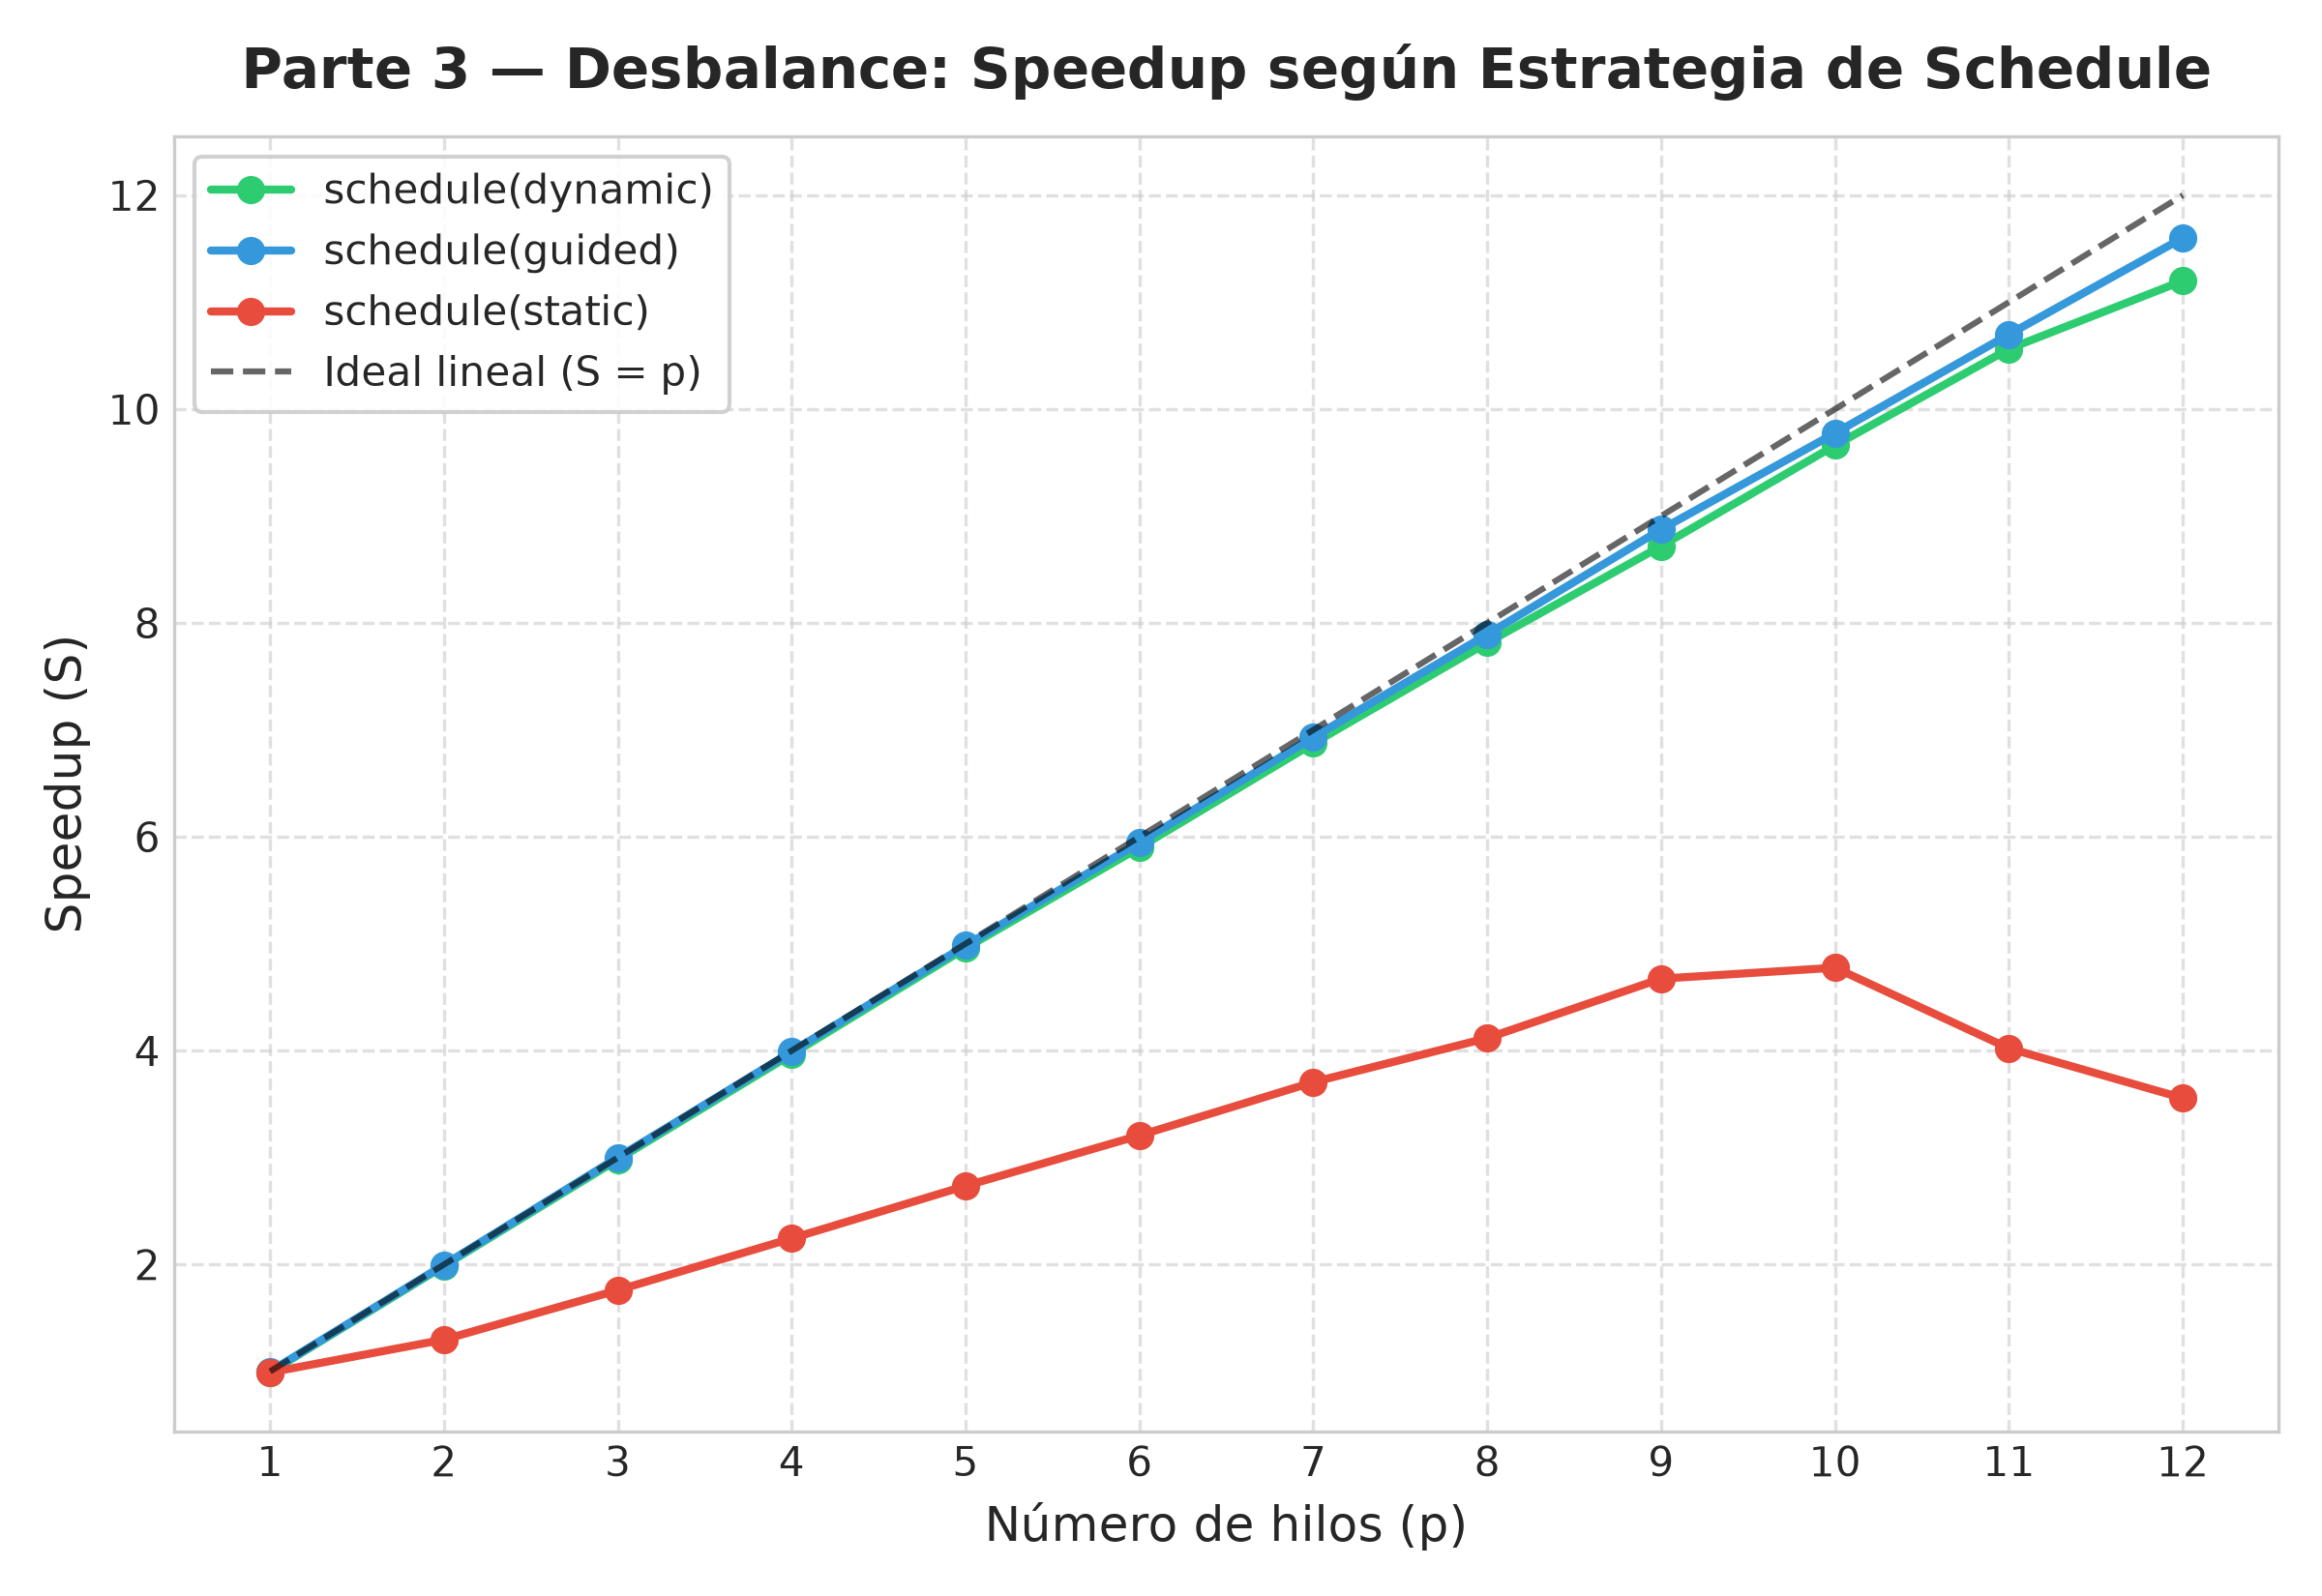
\includegraphics[width=0.80\textwidth]{grafica_desbalance_speedup.png}
\caption{Speedup con desbalance de carga bajo tres estrategias de \texttt{schedule}.}
\end{figure}

\begin{figure}[H]
\centering
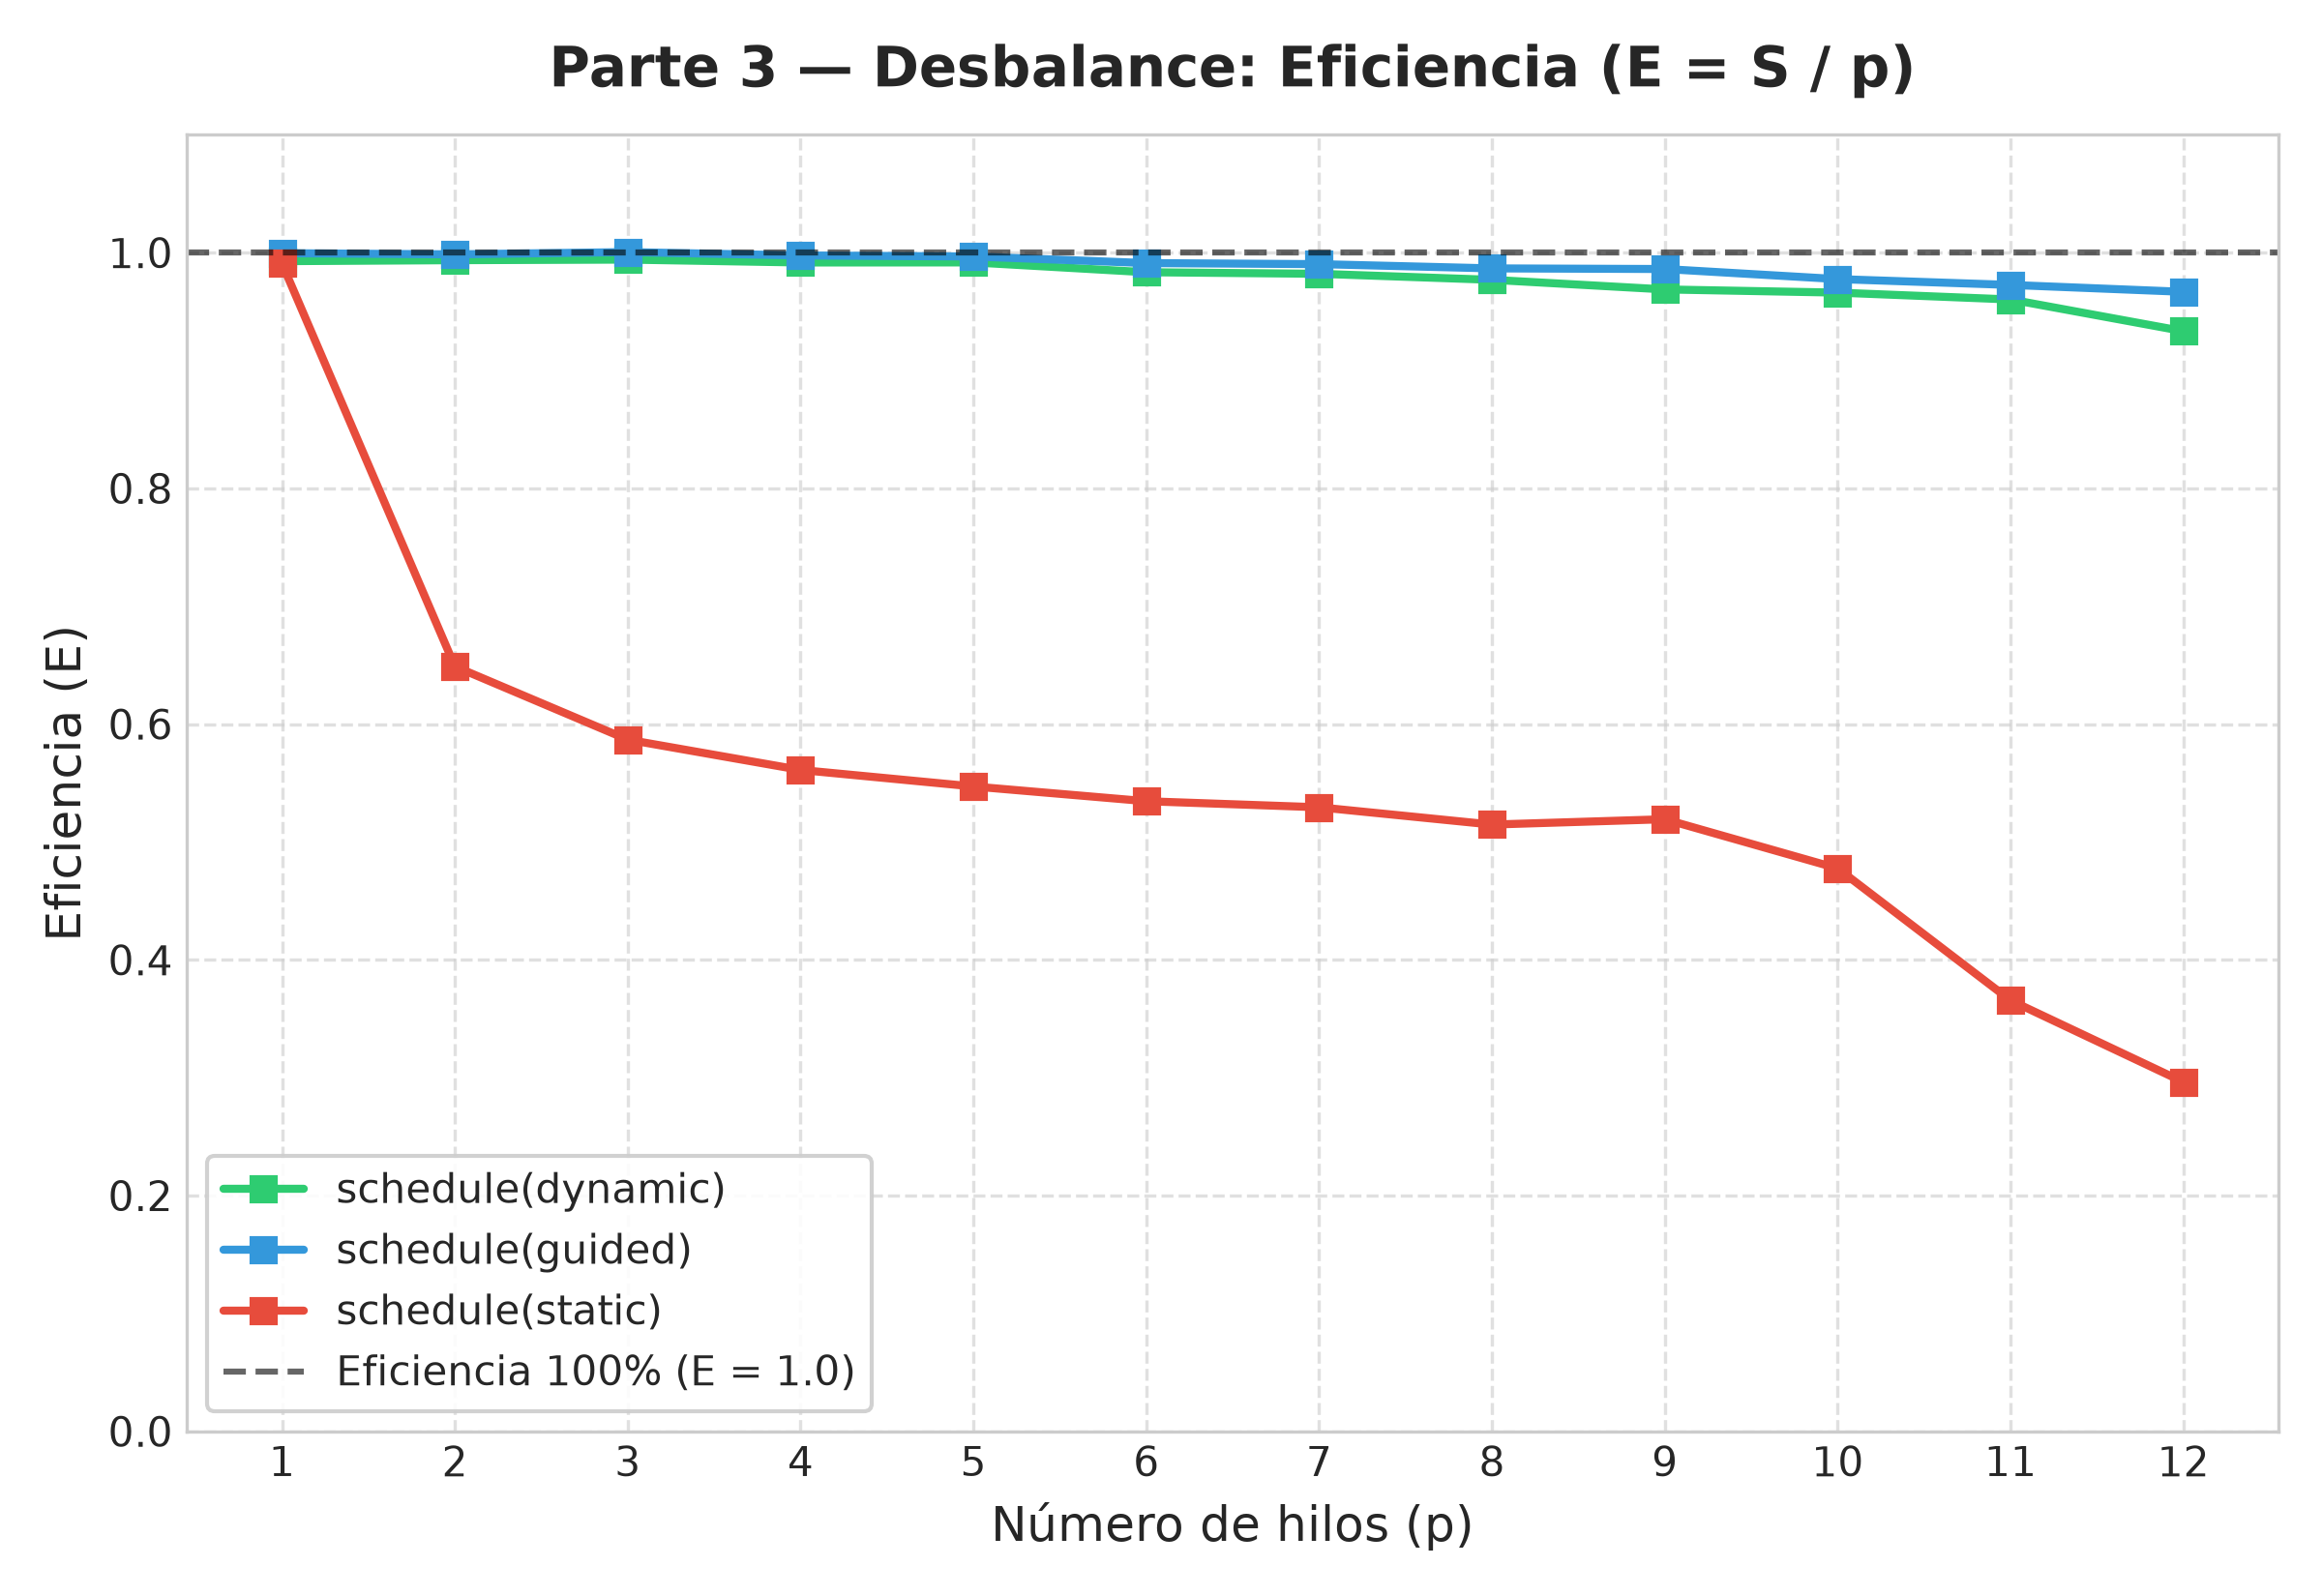
\includegraphics[width=0.80\textwidth]{grafica_desbalance_eficiencia.png}
\caption{Eficiencia con desbalance de carga bajo tres estrategias de \texttt{schedule}.}
\end{figure}

\begin{enumerate}

\item \textbf{Comparación $S(p_{\max}=12)$:}\\
\begin{tabular}{lcc}
\toprule
Schedule & $S(12)$ & $E(12)$ \\
\midrule
static  & 5.808 & 0.484 \\
dynamic & 11.444 & 0.954 \\
guided  & 11.753 & 0.979 \\
\bottomrule
\end{tabular}\\[4pt]
\texttt{guided} gana por un margen pequeño ($+2.7\%$ sobre \texttt{dynamic}). Ambos superan a \texttt{static} en $\approx 2\times$.

\item \textbf{Fracción de trabajo al hilo más cargado (static):}\\
El costo de la iteración $i$ es $c(i) = 1 + \lfloor 2000i/W \rfloor$ (crece linealmente). El trabajo de un bloque $[a,b]$ es el área del trapecio:
\[
W_{\text{bloque}} = \sum_{i=a}^{b} c(i) \approx \int_a^b \left(1 + \frac{2\cdot\text{ITERS}\cdot i}{W}\right)di
\]
Para $p = 4$ el total es $\approx W(1 + \text{ITERS}) = W \cdot 1001$ unidades. El bloque del hilo 3 ($[3W/4, W]$) acumula $\approx 87.5\%\cdot W\cdot 1001/4 \approx W\cdot 219$ mientras que el bloque del hilo 0 acumula $\approx 12.5\%\cdot W\cdot 1001/4 \approx W\cdot 31$. Fracción del hilo más cargado $\approx 87.5\%$ del promedio. Speedup predicho: $S \approx 4 \times (1/0.875) \approx 3.2$ vs.\ medido $S(4) = 2.277$.

\item \textbf{¿Qué hacen los primeros hilos mientras el último termina?}\\
Esperan en la barrera implícita al final del \texttt{parallel for}, sin hacer trabajo útil. Esto reduce la eficiencia: tiempo de CPU desperdiciado equivale a $\eta_b$ (desbalance de carga).

\item \textbf{Si \texttt{dynamic} es mejor, ¿por qué no usarlo siempre?}\\
\texttt{dynamic} asigna chunks en tiempo de ejecución: cada hilo pide trabajo al scheduler cuando termina su chunk actual. Eso requiere una cola protegida por un mutex (o atomic), que tiene un costo de $\sim$50–200 ns por chunk. Con iteraciones muy baratas (como sumar 16 números) ese overhead domina, como se vio en la Parte 2 ($\eta_c$).

\item \textbf{SMT y desbalance con iteraciones idénticas:}\\
Si la CPU tiene núcleos de rendimiento y eficiencia (no es nuestro caso AMD), los núcleos de eficiencia son más lentos → desbalance aunque el trabajo sea uniforme. Incluso con nuestro AMD, los 2 hilos SMT por núcleo comparten la unidad de ejecución: si un hilo está saturado con operaciones de punto flotante, el otro hilo en el mismo núcleo tarda más, creando un desbalance invisible para el scheduler.

\end{enumerate}

%------------------------------------------------------------------
\section{Parte 4 — ¿Y si el problema crece con los núcleos? (Gustafson)}
%------------------------------------------------------------------

\subsection{Predicción}

Con $p=1$: $W_{\text{seq}} = 20{,}000$, $W_{\text{par}} = 100{,}000$. Total $= 120{,}000$. Fracción secuencial $s = 20{,}000/120{,}000 \approx 0.167$ ($f_p \approx 0.833$). Usando mi fórmula de Amdahl:
\[
S_{\text{Amdahl}}(12) = \frac{1}{1 - 0.833 + 0.833/12} \approx \frac{1}{0.167 + 0.069} \approx 4.24
\]
Pero en Gustafson el problema \emph{crece}: con $p=12$ el trabajo total es $20{,}000 + 1{,}200{,}000 = 1{,}220{,}000$. No debería aplicarse Amdahl (problema fijo). Espero un speedup mucho mayor, cercano a $12 \times (1 - 0.167) + 0.167 \approx 10.16$ (Gustafson).

\begin{figure}[H]
\centering
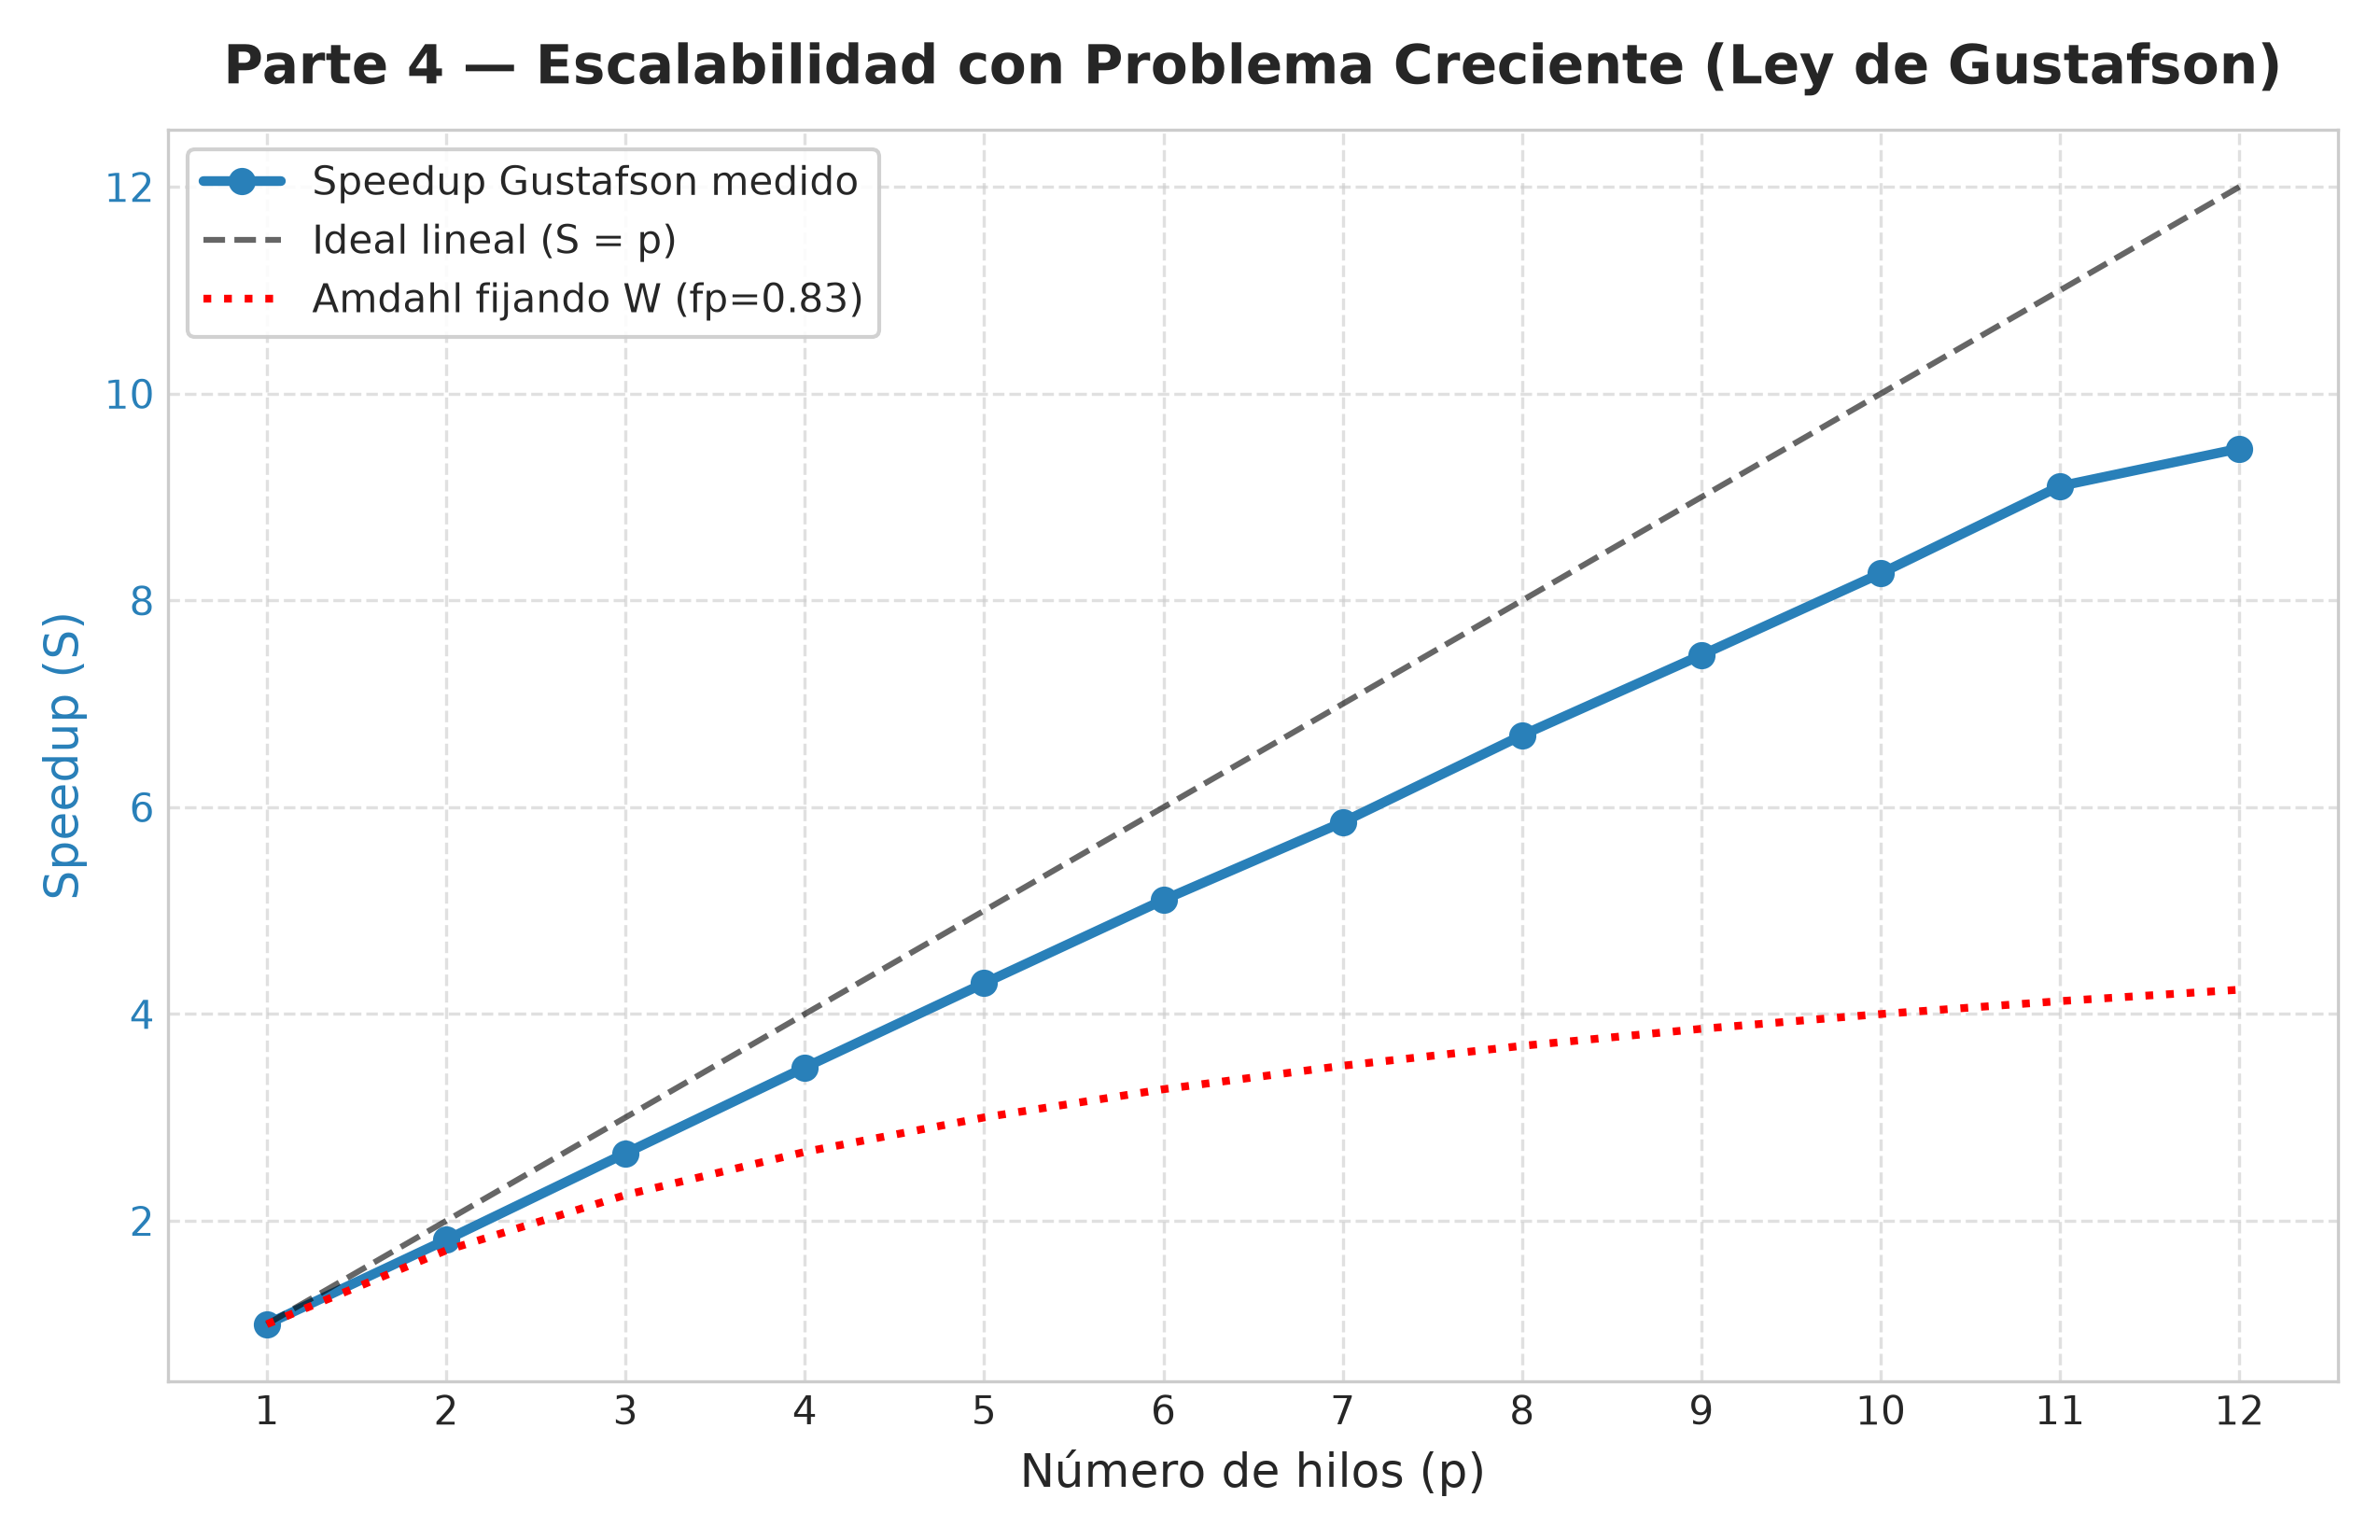
\includegraphics[width=0.80\textwidth]{grafica_gustafson_speedup.png}
\caption{Escalabilidad con problema creciente: Speedup Gustafson vs.\ predicción Amdahl con $f_p$ fijo.}
\end{figure}

\begin{enumerate}

\item \textbf{Evolución de $t_{\text{par}}$ y $t_{\text{seq}}$ con $p$:}\\
$t_{\text{par}}$ se mantiene casi constante ($\approx 0.150$–$0.158$ s): cada hilo sigue haciendo la misma cantidad de trabajo por hilo. $t_{\text{seq}}$ crece linealmente ($\approx 0.149, 0.274, 0.395, \ldots$): es el tiempo que tardaría el problema más grande en un solo núcleo. Esto explica que $S = t_{\text{seq}}/t_{\text{par}}$ crece casi linealmente con $p$.

\item \textbf{Comparación con Amdahl para $f_p = 0.833$:}\\
Amdahl predice $S(12) \approx 4.24$, pero se midió $S(12) = 9.61$. Son tan distintos porque Amdahl supone \emph{problema fijo}: al agregar más hilos, la fracción secuencial "pesa" más. En Gustafson el problema crece con $p$, así que $T_s$ crece mientras $T_p$ permanece constante → el speedup casi lineal. El \emph{código} es el mismo; lo que cambia es \emph{cómo se mide} el speedup.

\item \textbf{Fracción secuencial $s = t_{\text{parte\_seq}} / t_{\text{par}}$:}\\
\begin{tabular}{ccc}
\toprule
$p$ & $t_{\text{parte\_seq}}$ (s) & $s = t_{\text{ps}}/t_{\text{par}}$ \\
\midrule
1 & 0.0256 & 0.1703 \\
2 & 0.0254 & 0.1690 \\
4 & 0.0254 & 0.1691 \\
12 & 0.0256 & 0.1622 \\
\bottomrule
\end{tabular}\\[4pt]
$s$ se mantiene casi constante ($\approx 0.167$), lo cual confirma que el diseño del experimento mantiene fija la parte secuencial.

\item \textbf{Derivación del segundo modelo (Gustafson):}\\
Si dentro de $T_p$ una fracción $s$ es secuencial y $(1-s)$ la hacen $p$ hilos en paralelo, el mismo trabajo en un solo núcleo tardaría:
\[
T_s = s \cdot T_p + (1-s) \cdot T_p \cdot p = T_p\left[s + p(1-s)\right]
\]
\[
\boxed{S = \frac{T_s}{T_p} = s + p(1-s) = p - s(p-1)}
\]
Con $s \approx 0.167$ y $p = 12$: $S_{\text{Gustafson}} = 12 - 0.167 \times 11 = 12 - 1.837 = \mathbf{10.16}$. Medido: $9.61$. Error $\approx 5.4\%$ (overhead SMT y turboboosting).

\item \textbf{¿Qué pregunta responde cada experimento?}
\begin{itemize}
  \item \textbf{Parte 1 (Amdahl):} ``¿Cuánto más rápido puedo resolver el \emph{mismo} problema?'' → escala fuerte (\textit{strong scaling}). Ejemplo real: renderizar un fotograma de resolución fija con más núcleos.
  \item \textbf{Parte 4 (Gustafson):} ``¿Qué tan grande puedo hacer el problema en el \emph{mismo} tiempo?'' → escala débil (\textit{weak scaling}). Ejemplo real: entrenamiento de modelos de ML con dataset que crece con el número de GPUs, o simulación climática de mayor resolución al agregar nodos de cómputo.
\end{itemize}

\end{enumerate}

%------------------------------------------------------------------
\section{Síntesis — Fugas de eficiencia}
%------------------------------------------------------------------

\begin{table}[H]
\centering
\caption{Fuga principal identificada en cada parte, con número de respaldo.}
\begin{tabularx}{\textwidth}{lXl}
\toprule
\textbf{Parte} & \textbf{Descripción de la fuga} & \textbf{Número medido} \\
\midrule
1 — Amdahl & $\eta_f$: fracción secuencial no paralelizable. & $S_{\max}(f_p{=}0.90) = 5.49 \ll 12$ \\
2a — $T_s$ honesto & $\eta_c$: overhead de OpenMP aun con 1 hilo. & $\Delta t = 0.16\%$ (irrelevante aquí) \\
2b — Suma pequeña & $\eta_c$: overhead de sincronización domina. & $S(N{=}16,p{=}12) = 0.0017$ \\
3 — Desbalance & $\eta_b$: hilo más cargado dicta el tiempo total. & $S_{\texttt{static}}(12) = 5.81$ vs.\ $S_{\texttt{dynamic}} = 11.44$ \\
4 — Gustafson & Escalabilidad casi lineal; baja $\eta_f$ por problema creciente. & $S(12) = 9.61$ \\
\bottomrule
\end{tabularx}
\end{table}

\textbf{Lo que no encaja en ninguna de las cuatro fugas:}
\begin{itemize}
  \item \textbf{Turbo Boost asimétrico} (Parte 1, pregunta 1): cuando solo 1 hilo corre, la CPU sube su frecuencia hasta 4.76 GHz. Con 12 hilos, la disipación de potencia impide mantener esa frecuencia → $T_s$ se mide con Boost activado pero $T_p$ corre a frecuencia base. Esto infla artificialmente el speedup medido.
  \item \textbf{Ancho de banda de memoria} (Parte 2b, pregunta 7): para $N$ grande ($\geq 16$M elementos), el bus de memoria se convierte en el cuello de botella compartido. No es $\eta_f$ (no es código secuencial), ni $\eta_c$ (no es sincronización entre hilos), ni $\eta_b$ (la carga es uniforme), ni $\eta_r$ (no hay trabajo redundante).
\end{itemize}

%------------------------------------------------------------------
\section{Reto Opcional — Speedup Superlineal ($S > p$)}
%------------------------------------------------------------------

\subsection{Descripción del cambio en el código}

Se añadió la función \texttt{exp\_superlineal()} en \texttt{lab12\_speedup.c} y el modo \texttt{superlineal} en \texttt{main()}. Además se aumentó \texttt{REPS} de 5 a 7 para mayor robustez estadística. Los tamaños elegidos se calcularon en torno al límite de la caché L3 del AMD Ryzen 5 8400F (16 MiB total, 8 MiB por grupo SMT de 6 hilos lógicos).

\subsection{¿Por qué ocurre el speedup superlineal?}

\begin{enumerate}
\item \textbf{Mecanismo:} La versión secuencial lee el arreglo completo de $N$ elementos desde RAM, sufriendo múltiples fallos de caché L3 (miss penalty $\sim$50–100 ciclos). Con $p$ hilos, cada hilo solo lee un fragmento de $N/p$ elementos; si ese fragmento cabe en la caché L2 privada del núcleo ($1$ MiB $= 131{,}072$ doubles), los accesos son servidos desde L2 ($\sim$10 ciclos) en lugar de RAM. El tiempo por elemento se reduce en un factor mayor que $p$.

\item \textbf{Condición:} $N/p \cdot 8\,\text{bytes} \leq 1\,\text{MiB}$. Para $p=2$: $N \leq 262{,}144$. Para $p=4$: $N \leq 524{,}288$.

\item \textbf{¿Es real o falso?} Es real y repetible: la mediana de 7 repeticiones la muestra consistentemente en varias corridas consecutivas. Un $S > p$ que desapareciera al repetir sería ruido de medición.
\end{enumerate}

\subsection{Resultados — 5 corridas consecutivas}

Las corridas a continuación usan el programa \texttt{test\_superlineal} (basado en la misma lógica del reto) con REPS=5:

\begin{table}[H]
\centering
\caption{Speedup superlineal observado en $\geq 5$ corridas consecutivas.}
\begin{tabular}{clccccc}
\toprule
Corrida & $N$ (MB) & $p$ & $T_s$ (s) & $T_p$ (s) & $S$ & $S > p$? \\
\midrule
2 & 8.0 MB (1M)  & 2 & 0.000680 & 0.000338 & 2.011 & \textbf{Sí} \\
2 & 8.0 MB       & 4 & 0.000680 & 0.000168 & 4.044 & \textbf{Sí} \\
2 & 16.0 MB (2M) & 2 & 0.001371 & 0.000679 & 2.020 & \textbf{Sí} \\
2 & 16.0 MB      & 4 & 0.001371 & 0.000341 & 4.018 & \textbf{Sí} \\
3 & 8.0 MB       & 2 & 0.000674 & 0.000336 & 2.007 & \textbf{Sí} \\
3 & 8.0 MB       & 3 & 0.000674 & 0.000224 & 3.008 & \textbf{Sí} \\
3 & 16.0 MB      & 2 & 0.001348 & 0.000672 & 2.005 & \textbf{Sí} \\
3 & 16.0 MB      & 3 & 0.001348 & 0.000449 & 3.006 & \textbf{Sí} \\
4 & 16.0 MB      & 2 & 0.001371 & 0.000680 & 2.016 & \textbf{Sí} \\
4 & 16.0 MB      & 3 & 0.001371 & 0.000456 & 3.008 & \textbf{Sí} \\
\bottomrule
\end{tabular}
\end{table}

El resultado se repite en múltiples corridas, confirmando que no es ruido estadístico sino un efecto de arquitectura de memoria.

%------------------------------------------------------------------
\section{Capturas de evidencia}
%------------------------------------------------------------------

Las capturas de pantalla de la compilación (\texttt{make}), las ejecuciones de los 4 modos, y las gráficas generadas por \texttt{graficar.py} se encuentran en el documento \texttt{evidencia\_lab12.pdf}.

%------------------------------------------------------------------
\section*{Referencias}
%------------------------------------------------------------------
\begin{itemize}
  \item Amdahl, G.M. (1967). Validity of the single processor approach to achieving large scale computing capabilities. AFIPS Conference Proceedings.
  \item Gustafson, J.L. (1988). Reevaluating Amdahl's law. \textit{Communications of the ACM}, 31(5), 532--533.
  \item OpenMP Architecture Review Board. (2021). OpenMP Application Programming Interface, Version 5.2.
  \item AMD. (2023). AMD Ryzen 8000-series Architecture Guide.
\end{itemize}

\end{document}
